\documentclass[letterpaper, 12pt, dvips]{mitwpl}
\usepackage{pstricks}
\usepackage[novbox]{pdfsync}
\setlength{\headheight}{14.5pt}
\usepackage{graphicx}

%%% BEGIN DOCUMENT
\begin{document}

\papertitle{LingSync: A Free Tool for Creating and Maintaining a Shared Database For Communities, Linguists and Language Learners}

\firsttitle{\LARGE LingSync: \\[.2ex]\Large   A Free Tool for Creating and Maintaining a Shared Database For Communities, Linguists and Language Learners}
\runningtitle{iCampo/LingSync}

\author{MaryEllen Cathcart$^{a,b}$\\ Gina Cook$^b$\\ Theresa Deering$^{b,c}$\\ Yuliya Manyakina$^{d}$\\Gretchen McCulloch$^d$\\Hisako Noguchi$^e$}
\runningauthor{Cathcart et al.}
\institution{$^a$University of Delaware $^b$iLanguage Lab $^c$Visit Scotland $^d$McGill University$^e$Concordia University}
\ackfn{iCampo: Un aplicaci\'on de colecci\'on de datos ling\"u\'isticos\\

We would like to thank the CAML participants for their comments and questions, 
Android Montr\'eal and Javascript Montr\'eal for their comments and feedback on aspects of LingSync presented at meet-ups,
as well as Montreal's start-up community for permitting linguists to immerse themselves in the software community, 
without which we would not have discovered technologies  so well-suited to a field database.
We would also like to express our deep thanks to Tobin Skinner,
Josh Horner,
Elise McClay,
Louisa Bielig,
Joel Dunham,
Brian Doherty, 
Gay Hazan,
Oriana Kilbourn,
Rakshit Majithiya,
Kim Dan Nguyen,
Pablo Duboue, as well as countless other open source software developers whose code directly or indirectly helped build LingSync to what it is today.
We would like to thank Mathieu Legault for his substantial financial contributions which made LingSync advance far quicker than expected,
as well as the granting agencies which supported the students who have doubled as field work research assistants and interns on the project. 
%Lastly we would like to thank our significant others for their support and patience: without them,
%our passion for better data experiences would have remained just that,
%a passion and not a reality.
}

\maketitle

%\renewcommand*\abstractname{Resumen}
%
%\begin{abstract}
%Lorem ipsum dolor sit amet, lectus faucibus, vitae tortor velit ut dolor integer, nunc sapiente mi, mauris nam magna, gravida et eu quisque. Etiam nibh mi tincidunt, libero euismod sed consectetuer amet, nam eget donec scelerisque sem sodales, curabitur et ut imperdiet libero leo pulvinar. Eros ipsum consectetuer donec imperdiet, dictum aliquet ac sollicitudin dui. Amet magna. Nunc nam. Pellentesque aut vestibulum, neque neque lacus quisque, curabitur bibendum fringilla pede magna non sociis, tempus gravida orci neque dictumst donec, etiam sit. Lorem ipsum dolor sit amet, lectus faucibus, vitae tortor velit ut dolor integer, nunc sapiente mi, mauris nam magna, gravida et eu quisque. Etiam nibh mi tincidunt, libero euismod sed consectetuer amet, nam eget donec scelerisque sem sodales, curabitur et ut imperdiet libero leo pulvinar. Eros ipsum consectetuer donec imperdiet, dictum aliquet ac sollicitudin dui. Amet magna. Nunc nam. Pellentesque aut vestibulum, neque neque lacus quisque, curabitur bibendum fringilla pede magna non sociis, tempus gravida orci neque dictumst donec, etiam sit. Lorem ipsum dolor sit amet, lectus faucibus, vitae tortor velit ut dolor integer, nunc sapiente mi, mauris nam magna, gravida et eu quisque. Etiam nibh mi tincidunt, libero euismod sed consectetuer amet, nam eget donec scelerisque sem sodales, curabitur et ut imperdiet libero leo pulvinar. Eros ipsum consectetuer donec imperdiet, dictum aliquet ac sollicitudin dui. Amet magna. Nunc nam. Pellentesque aut vestibulum, neque neque lacus quisque, curabitur bibendum fringilla pede magna non sociis, tempus gravida orci neque dictumst donec, etiam sit. 
%
%\end{abstract}



\renewcommand*\abstractname{Abstract}

\begin{abstract} 
LingSync is a free,
open source data management system built for field linguistics teams.
It allows teams to securely enter,
store,
organize,
annotate,
and share linguistic data.
The application is accessible on any device; 
not only on laptops (Mac,
Linux,
Windows,
ChromeBooks) but also touch tablets or mobile devices (Android and iPhone/iPad).
 It is suitable for both online and offline use,
yet,  
data is syncable and sharable with other researchers as well as the language community.
 Team members use the application not just to view and modify data,
but also to analyze and discuss the data.
The system also has a simple and friendly user interface,
allowing users to drag and drop data (audio,
video,
text),
or record audio/video directly into the database.
The application has import and export capabilities for multiple file types.
LingSync was designed from the ground up to conform to E-MELD and DataOne data management best practices,
an important requirement for any application used by data collection projects funded by granting agencies.
Finally,
the application is designed to be intuitive and theory free,
so it is not necessary to be a field linguist, or programmer to figure out how it works.
LingSync is hosted on cloud servers so that users can use it without knowing how to set up their own servers,
but it also has an installation guide for server administrators so organizations can run their own instance of LingSync. Not only is its source code 100\% open, LingSync's development is also 100\% open and driven by the research assistants of field work teams who use the application.
\end{abstract}


\section{Background}
\label{sec:background}

\cite{Thieberger:2012} identifies ``a need for research into existing and emerging methods and development of tools both for creating linguistic data and then for making it useful.'' 
In this paper we hope to demonstrate how the LingSync project embodies Thieberger's call to action. Section \S \ref{sec:background} provides some background to the project including why \S \ref{sec:why} LingSync was created despite numerous existing solutions, and the data management best practices \S \ref{sec:design} underlying LingSync. 
Section \S \ref{sec:what} discusses LingSync's core \S \ref{sec:core} functionality as well as how LingSync empowers teams  with plugins \S  \ref{sec:plugins} to reuse and repurpose existing resources and software libraries. Section \S \ref{sec:use} discusses how teams are currently using LingSync, and celebrates LingSync's  growing community of over 300 users in just 1.5 years since the project was launched at CAML. Section \S \ref{sec:conclusion} summarizes  the paper.

\subsection{Why LingSync was created}
\label{sec:why}
\subsubsection{The need}

LingSync was conceived out of the needs of language researchers doing
fieldwork, or other large scale data collection, 
often in a partnership with language community members, 
and unlike professional field linguists, 
 not on a full-time basis but rather as one of many other tasks (including, but not limited to, teaching, grading, researching and preparing publications).
Linguistic fieldwork frequently occurs where a stable connection to the internet is not guaranteed.
In addition,
it frequently involves a group of researchers, research assistants and native speakers contributing to building a single data collection.
An ideal linguistic database should therefore work both online and offline \citep[p.1556]{Wittenburg:2006}, as well as
make it easy to share and integrate data resources,
not only among researchers but also with the language community \citep{Good:2012, Thieberger:2012}.


\subsubsection{Other programs: pros and cons}


There are several existing programs designed specifically for storing linguistic data; however,
none of them fully satisfies a field work team's need for robust,
collaborative,
multi-platform data annotation and organization,
both online and offline.
For example,
there are web-based databases which allow collaboration and sharing research with the language community,
such as 
the Yurok Documentation Project \citep{Yurok:2001:Online},
 Karuk Dictionary and Texts \citep{Karuk:2009:Online},
the Washo Project \citep{Washo:2005:Online, WashoMobile:2008:Online, Cihlar:2008}, 
and the Online Linguistic Database (OLD) \citep{OLD:2010:Online} to mention only a few. 
However, they only work online,
making them unusable for editing or searching the data while in the field with limited or no internet access.
There are also non-web-based software programs such as ToolBox \citep{ToolBox:2003:Online} 
and FLEx/FieldWorks,
\citep{FLEx:2011:Online}
which are often the best tools for annotating
data and organizing data into various forms of deliverables  
including a corpus,
grammar and lexicon.

However, these offline tools were not designed for collaboration. 
Field workers generally each enter data on a single computer,
and merge data later when online,
 meaning that collaboration in these tools must use an ad-hoc mechanism which works similarly to DropBox, e-mail (or in an industry setting, a version control system such as SVN or Git)
as well as transformation scripts to permit multiple users to combine their data structures with other field workers who work on related projects.
One of the most difficult problems to overcome is that 
these tools only run on platforms which are popular among professional field workers  (usually Windows and sometimes Linux), but 
not Mac or mobile devices, and can require too much training in the context of field linguistics labs with a high turn over (or field methods courses) where team members do not devote 100\% of their time to data management \citep{Butler:2007}.

There are many other ad-hoc solutions which are not specifically designed for linguistic field work, including general purpose database software such as FileMaker Pro,
which can be customized for the purpose of language research.
However,
this incurs the same problems as other offline tools,
while additionally a programmer or programming-linguist must be hired to customize the software for the purpose of linguistic research.

None of the linguistic database software surveyed above provided a modern user experience.
The number of clicks required, the delay between actions, and inability to efficiently browse the data did not meet current
Human Computer Interaction and Software Engineering best practices, 
not to mention the expectations of users who were accustomed to using professionally crafted, data-heavy software such as FaceBook, WordPress, Evernote and Google. %to mention only a few.
In addition to core functionalities, field linguistics teams have very limited resources. 
A good user
experience is absolutely crucial to maximize the amount of high-quality data produced for the budgeted research hours \citep{Palmer:2009}. 
LingSync grew
out of discussion with a number of field work labs who had improvised their own ad-hoc systems, 
(despite being aware of the existing packaged professional field work solutions mentioned above), 
and programming-linguists who worked in the software industry and knew that the fabric of technology had changed significantly enough to make it feasible to build a system which could reconcile many of the previously irreconcilable constraints.


\subsubsection{Technological background: why we can make this now} 

While the rest of this paper (with the exception of Plugins \S \ref{sec:plugins}) targets a field linguist audience, a discussion of LingSync is incomplete without some discussion of why LingSync is unique among field databases.

LingSync is actually only an open ended recursive data schema (\ref{ex:intelligible}) % (Appendix \S \ref{appendix:datumjson}), 
and a few simple Node.js web services. All of the heavy lifting of the system is done by CouchDB. CouchDB is an open source  project which began in 2005 and matured in 2010, with continuing exciting additions each year following. 

CouchDB  solves important problems for field linguists, such as the ability to change their  data structure (\ref{ex:Irreconcilable}a) as their field database evolves\footnote{CouchDB stores data as JSON which is the equivalent of XML, meaning that it is more similar to the flexibility of ToolBox and ELAN but yet still has the ability to be extremely structured like FLEx.} 
%CouchDB's map reduce functions are a powerhouse for searching highly structured diverse data without pushing round data into square holes. LingSync add sample `bots' to CouchDB so teams can clean and restructure data to follow and update to new conventions and new analyses of the data.} 
and matures. CouchDB was designed for collaboration  (\ref{ex:Irreconcilable}b)\footnote{All documents are versioned, so each time a team member saves a record, it gets a new version.} 
as well as to work offline.\footnote{CouchDB knows how to keep two or more computers in complete sync permitting team members to go offline with a full copy of their data and come back online again without manually merging the data.}
 With CouchDB under the hood, teams can prototype iPhone apps  and other useful results \emph{with} language communities (\ref{ex:Irreconcilable}c) \emph{while} doing field work, without waiting\footnote{CouchDB is, oddly enough, not just a database, but also a server. It is able to serve data at a unique URL without the need to write a custom API.}
  to export their data to another tool. Yet, all the permissions\footnote{CouchDB uses authentication tokens which can be shared across different client apps, meaning that if the user logs LingSync in one window, they can access the data in another app in another window (an experience very similar to Gmail and Google Docs). LingSync adds additional measures discussed in Sharing \S \ref{sec:sharingactivityfeeds} below.}
 of the data are still enforced, meaning that the same database can both serve primary audio and video \citep{Pfeiffer:2010} data, but also keep it private until it has been polished for community use. CouchDB can look like a webpage, with colors and buttons (\ref{ex:Irreconcilable}d) but yet, the team's power users\footnote{Most labs we talked with had someone in their lab who had learned Python to be able to transform data. CouchDB has a console where you can script transformations to your data and visually see the results immediately. Being in a web technology and using Javascript, research assistants can copy paste their way to new scripts and other useful internal tools for the team, with no need to find a computer science student and then teach them the subtitles of linguistic data to ensure that the way they clean data doesn't introduce errors. } 
 can seamlessly explore data in its true form, and even edit and customize existing LingSync scripts to clean and transform data into new shapes for analysis and export.

\begin{exe}
\ex  Previously Irreconcilable Constraints

\begin{tabular}{lllcl}
&& & Year & Technology \\\hline\hline
a. & highly structured, & yet flexible & 2005 & NoSQL\\\hline
b. & collaborative, & yet offline  & 2012 &  IndexedDB\\\hline
c. & open data enabled,  &yet facilitate respect the wishes  & 2012 & CORS \\
&&  of language community members \\\hline
d. & easy to use,  &yet provides a seamless context switch  & 2005 & Chrome DevTools  \\
&& to a power-user friendly interface && CouchDB
\end{tabular}
\label{ex:Irreconcilable}
\end{exe}


%More  details are provided in  appendix \S \ref{appendix:technology}.

\subsection{Design principles} 
\label{sec:design}

The principal goal of LingSync is to help language researchers collect and organize linguistic data and to facilitate collaborative research work. Main objectives are outlined in (\ref{ex:objectives}). 
LingSync is designed so that it requires no training nor complicated set-up for data categories, and takes no time to add new categories.  The application does not include any theoretical constructs that must be tied to the data.  The application allows data fields and categories to develop organically as data collection proceeds. Researchers are able to add and change their fields and categories for the data at any point. 




\begin{exe} 
\ex Objectives

\begin{xlist}
        \ex  A self-explanatory, easy-to-use user interface so that researchers can understand and start using the application without laborious training about the software.
        \ex Customizable data entry fields to accommodate particular requirements of a research.  
        \ex  Data sharing, protection and integration functions to facilitate collaboration among researchers and between researchers and language consultants. 
    \end{xlist}
\label{ex:objectives}
\end{exe}


In addition to the user driven objectives in (\ref{ex:objectives}), LingSync was designed to comply with the recommendations from %in two respects: Data Documentation and Data Management. Data documentation will be evaluated following 
E-MELD Best Practices in Digital Language Documentation,\footnote{http://emeld.org/school/what.html} and %data management following 
DataONE Primer on Data Management.\footnote{http://www.dataone.org/sites/all/documents/DataONE\_BP\_Primer\_020212.pdf}
The following section discusses the design of LingSync with respect to E-MELD %and DataONE 
best practice recommendations. 


\subsubsection{E-MELD Best Practices in Digital Language Documentation}
\label{sec:documentation} 

E-MELD describes seven common problems in digital language documentation identified in \cite{Bird:2003} and recommends solutions. LingSync's implementation of these solutions is included below.

\begin{description} 

\item {\bf Content}: Data is annotated and described using consistent terminology.  

%Terminological conventions used to annotate data are all too often not explicitly defined in the database. 
%Members of a research team might use the same terms in different ways, or use different terms to mean the same thing, depending on their theoretical background or expertise in the language being documented. 
%This often result in terminological inconsistency and ambiguity within a database, which is hard for computers to resolve.
LingSync allows users to design their annotation conventions per corpus and makes these conventions available as a help text next to each field of each record of the corpus, ensuring that conventions are never far away, and reducing tension among team members.
Although a consistent  terminology is necessary for cross-corpora integration  \citep{Schalley:2012}, the app's primary users require that it to adapt to a particular linguistic framework or theoretical construct. As such, LingSync permits researchers to use open ended categories for annotation. 
To enable consistency, open-ended typeahead drop-downs, shown in (\ref{ex:consistent}) permit team members to see what has previously been used, and optionally add new tags and categories without needing to leave the data entry interface.


\begin{exe} 
\ex Data is open-ended, yet consistent

 \centering
    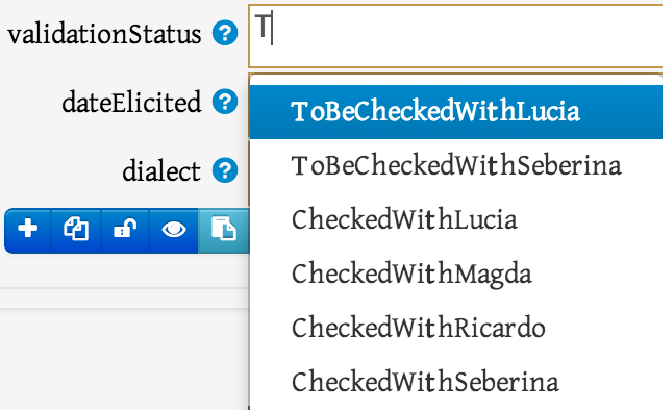
\includegraphics[width=0.35\textwidth]{typeaheadForPreviousCategories}

\label{ex:consistent}
\end{exe}

\item {\bf Format}: Data is intelligible regardless of the types of operating system. 
 
%The use of non-standard (non-ASCII) fonts is sometimes inevitable in linguistic data, however, not all applications support non-ASCII fonts. Data could also become unintelligible due to the file formats that are incompatible with other applications or operating systems. 
LingSync is written in Javascript and web technologies which permit the application to be 100\% Unicode, including support for right to left orthographies as well as IPA symbols. LingSync data is stored as plain text, and exportable in human readable formats including JSON, LaTeX, CSV, and XML, all of which are non-proprietary and compatible with applications commonly used in linguistic data collection and documentation. LingSync runs on PC, Linux and Mac OS, as well as on newer platforms such as Android, ChromeBook and iPad.

\begin{exe} 
\ex Data is stored as plain text in Unicode

 \centering
    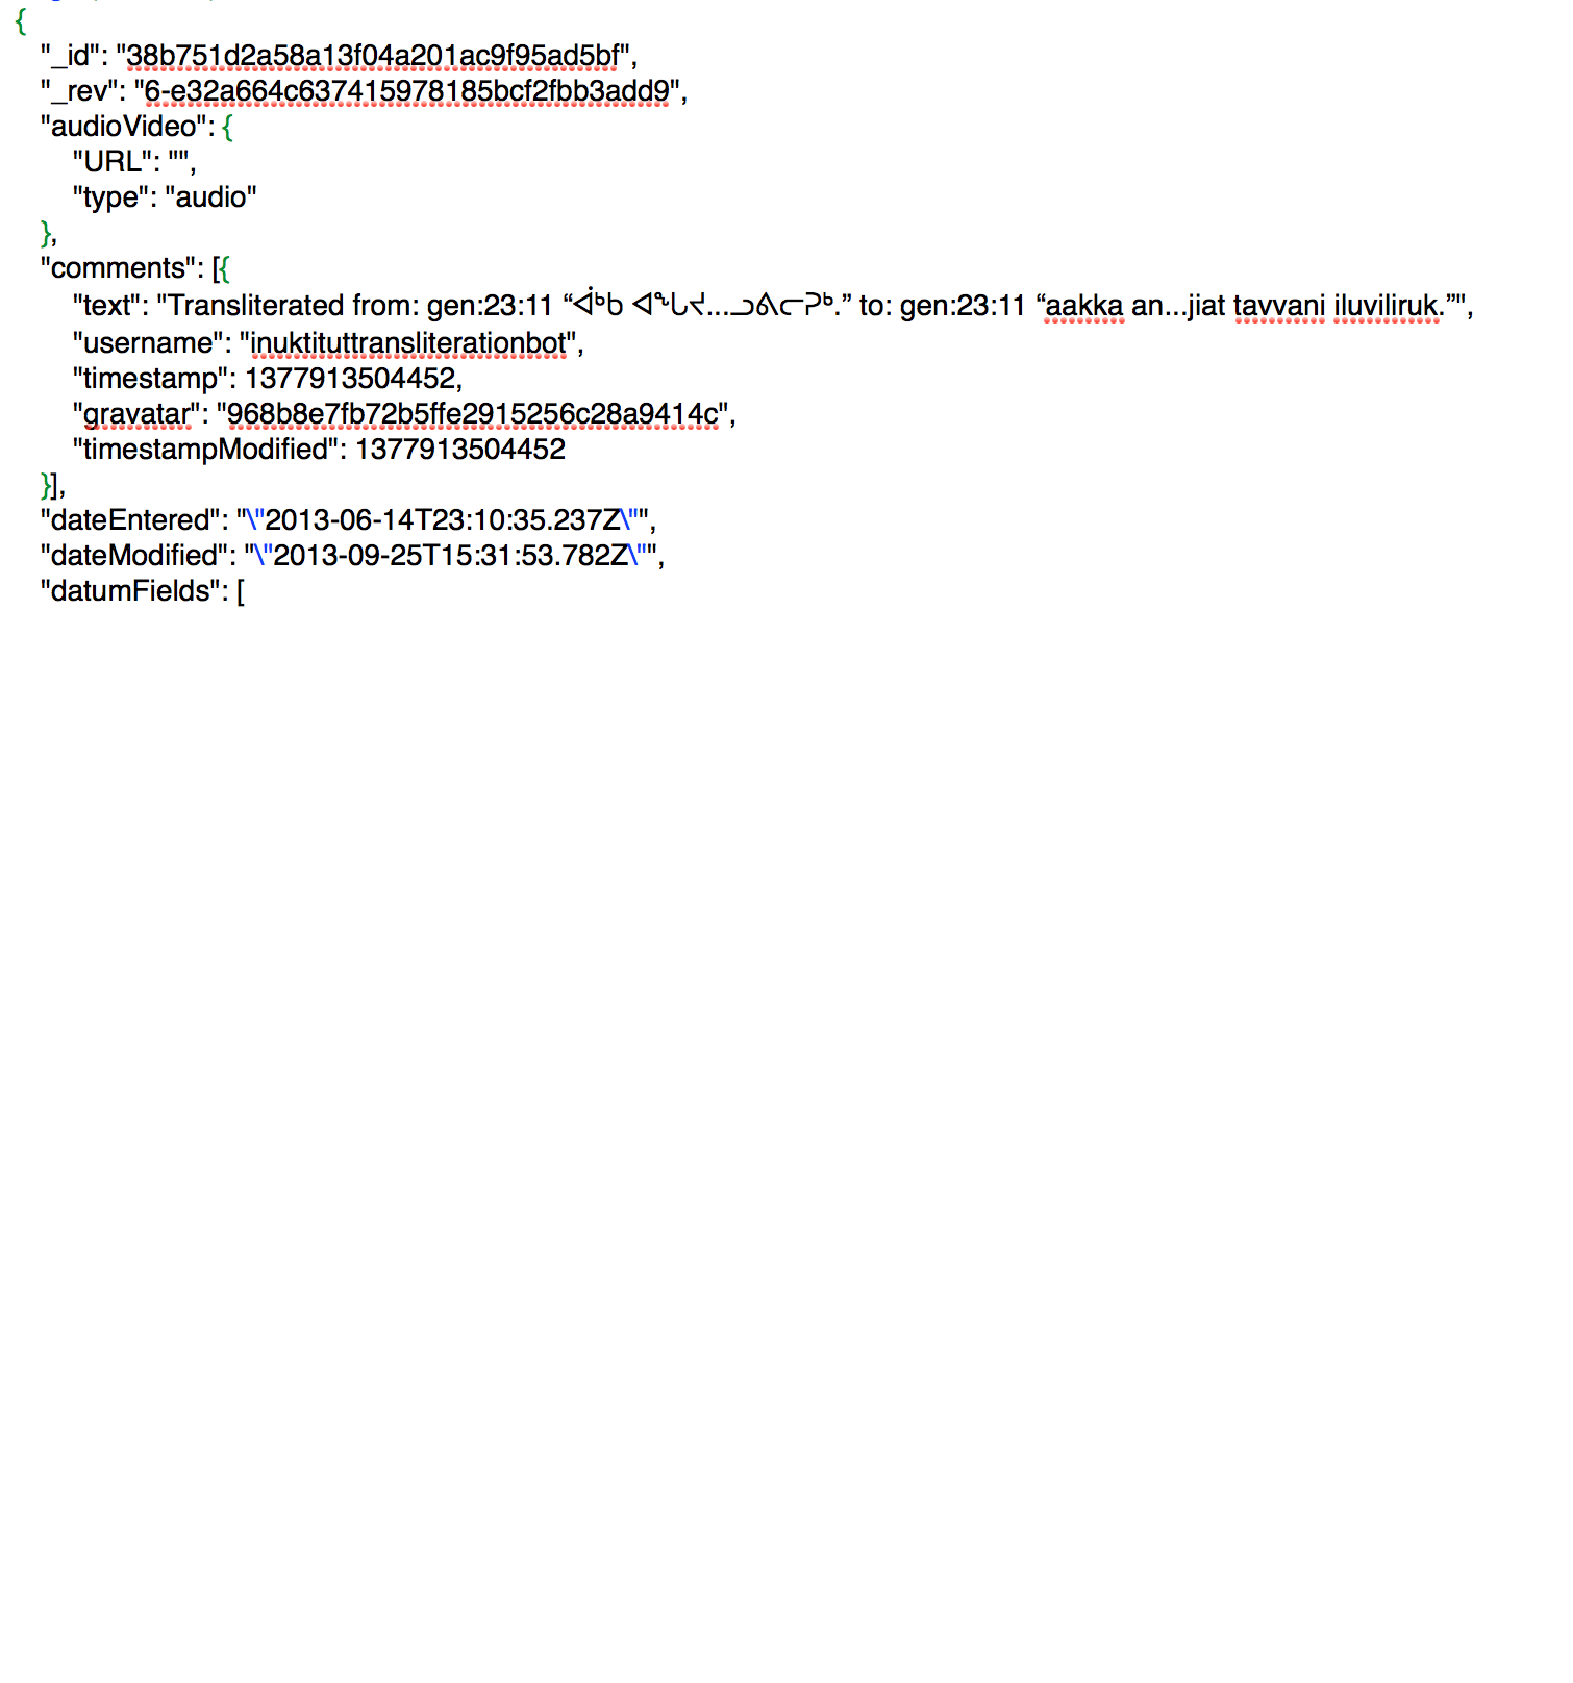
\includegraphics[width=0.8\textwidth]{dataIsPlainTextUnicode}

\label{ex:intelligible}
\end{exe}


\item {\bf Discovery}: Data is searchable and discoverable. 
 
Inside LingSync, data is searchable via keywords, or within specific fields, using either simple strings or regular expressions (\ref{ex:searchable}). 
%The search module is capable of performing intersective or union search of the data using any of the fields. 
\begin{exe} 
\ex Data is searchable both for normal users, and for power users

 \centering
    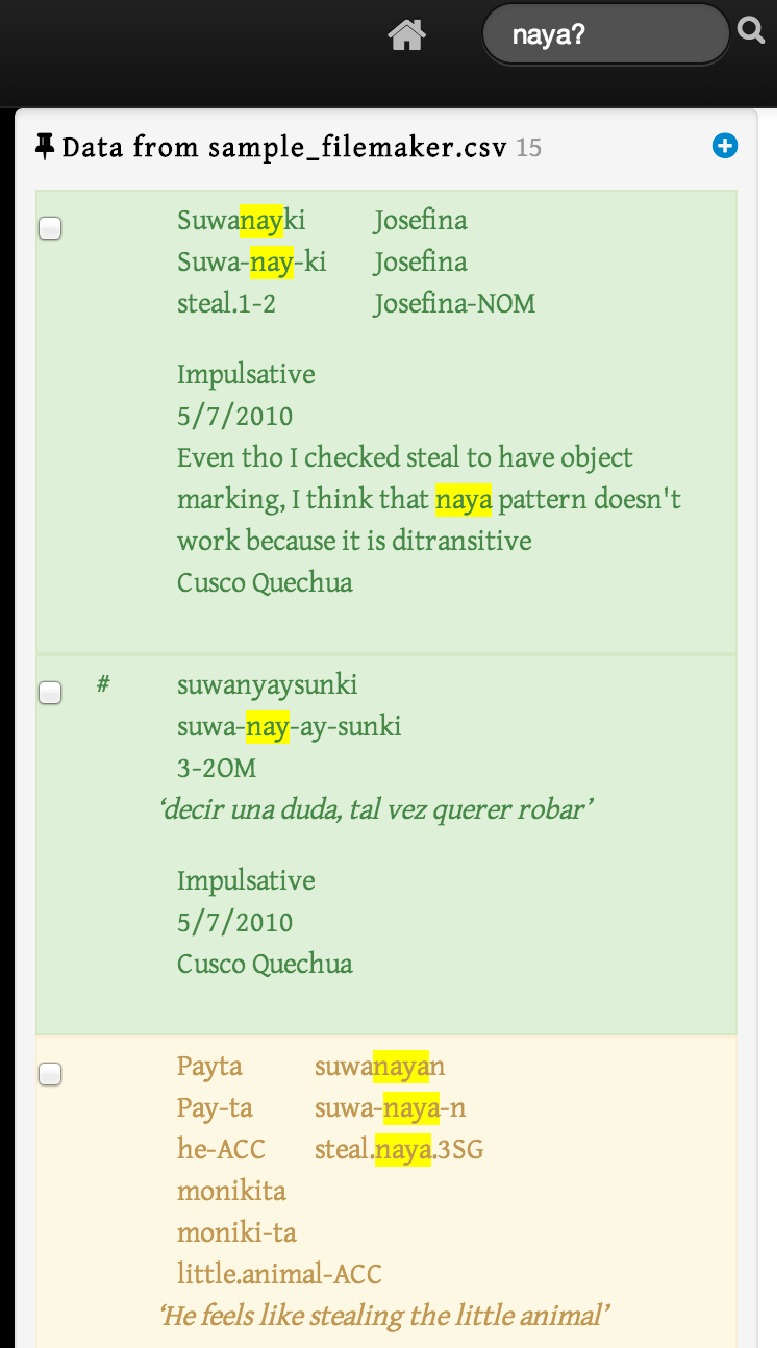
\includegraphics[width=0.4\textwidth]{searchable}

\label{ex:searchable}
\end{exe}

%It is often hard to find relevant linguistic data with standard search engines such as Google and Yahoo.  
Public  corpora are   (\ref{ex:discoverable}a) are SEO enabled, and can be exported to the OLAC linguistic search engine.\footnote{ http://linguistlist.org/olac/index.html 
\hspace{.2cm}http://www.language-archives.org/documents/implement.html\#conventional} Corpus administrators  control what is public, down to each field of each data record. Sensitive information can even be encrypted in the database, and displayed masked (\ref{ex:discoverable}b), meaning that the entire corpus can be exported and shared without combing the data to black out sensitive information. 

\begin{exe} 
\ex a) Data can be search engine discoverable, b) fields can even be public yet masked 

\hspace{-1.5in}
 \centering
   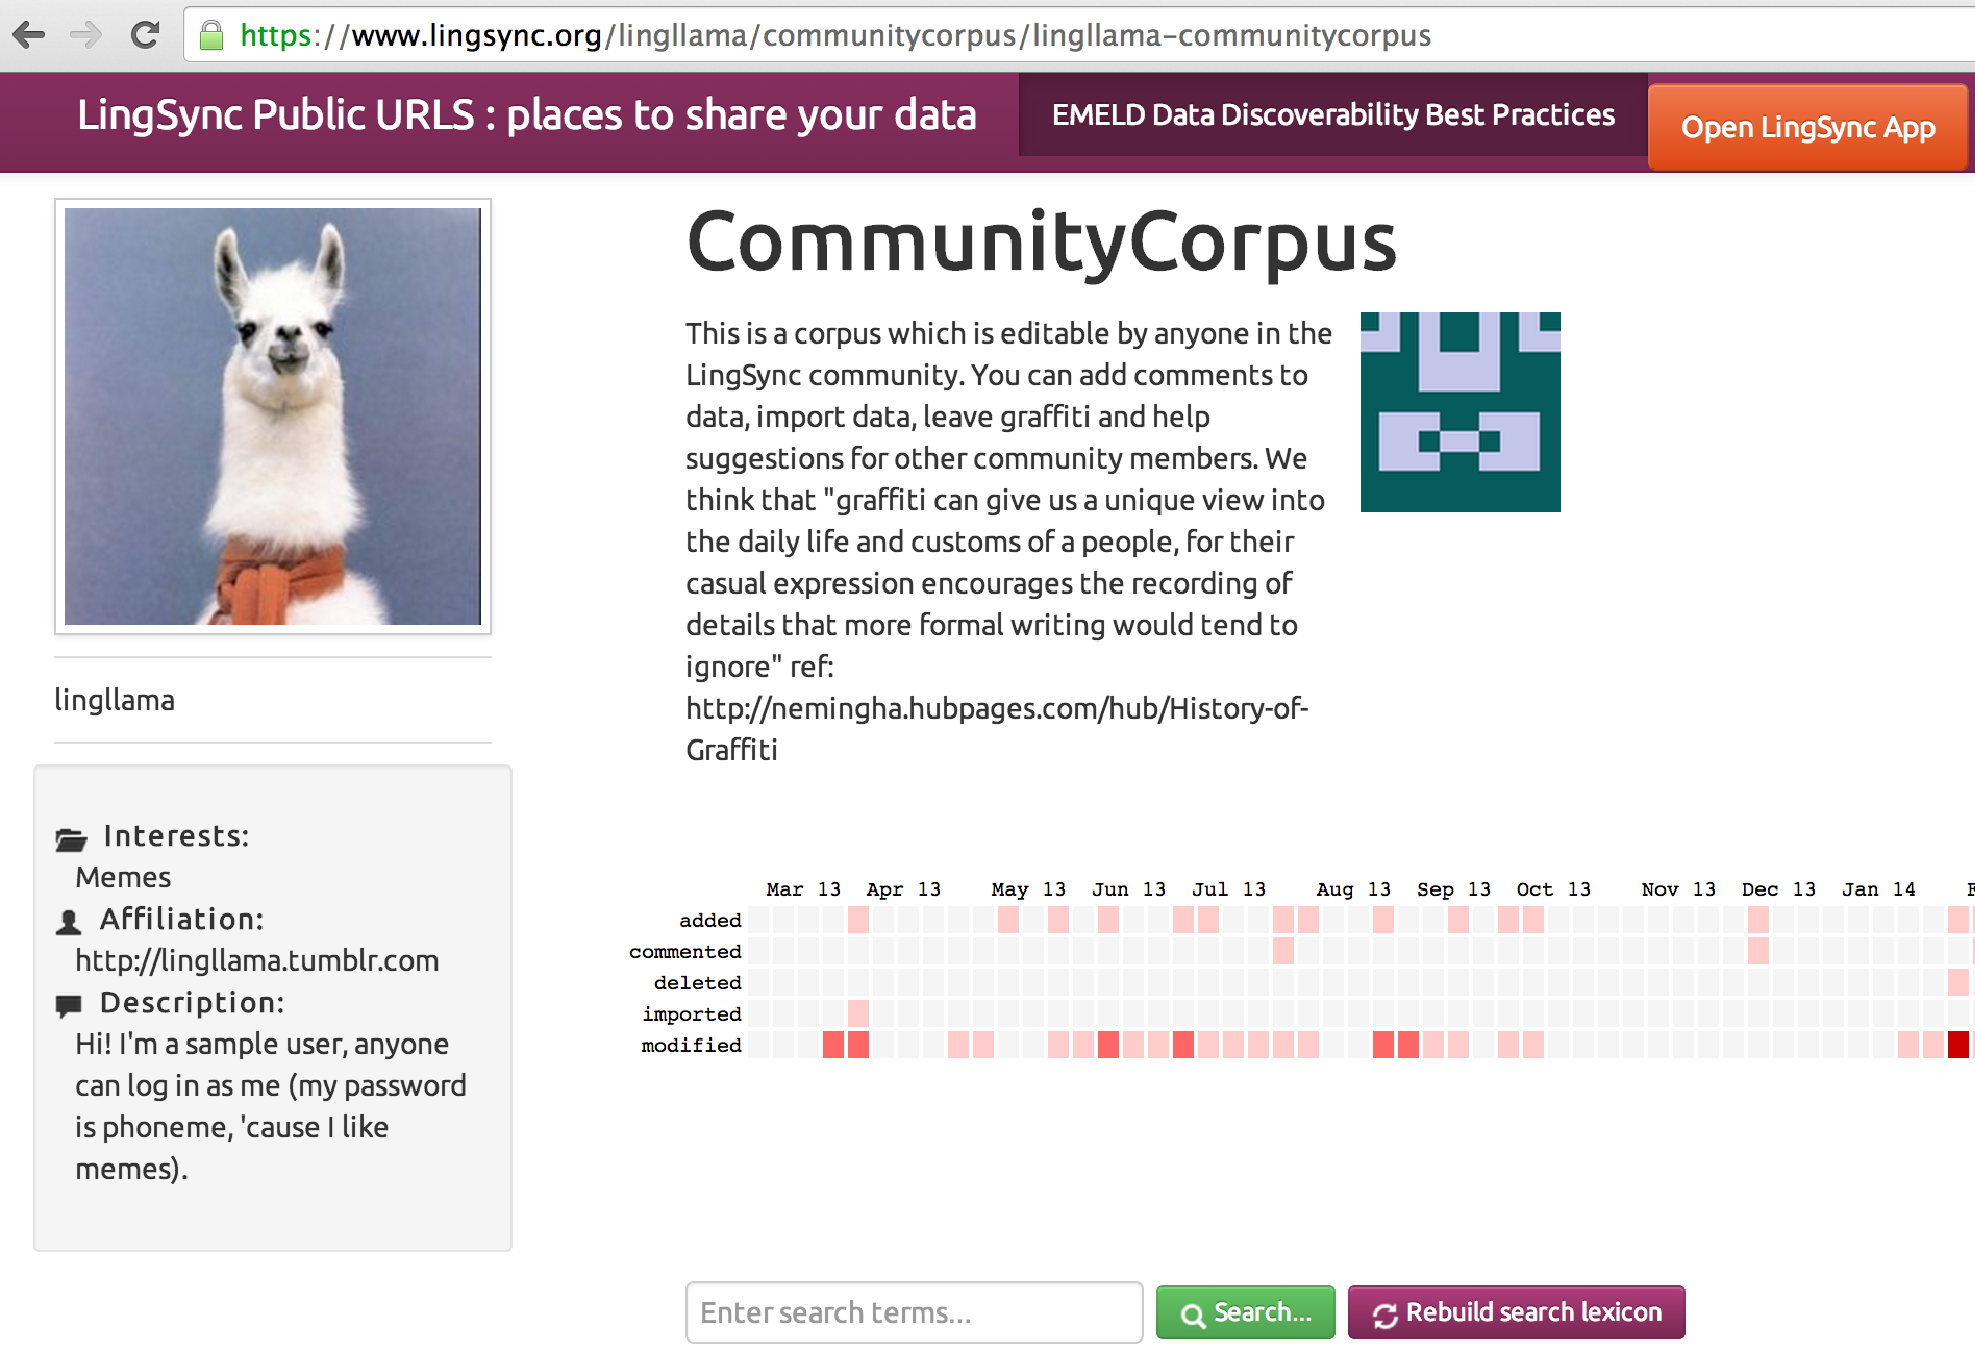
\includegraphics[width=0.4\textwidth]{discoverable}
   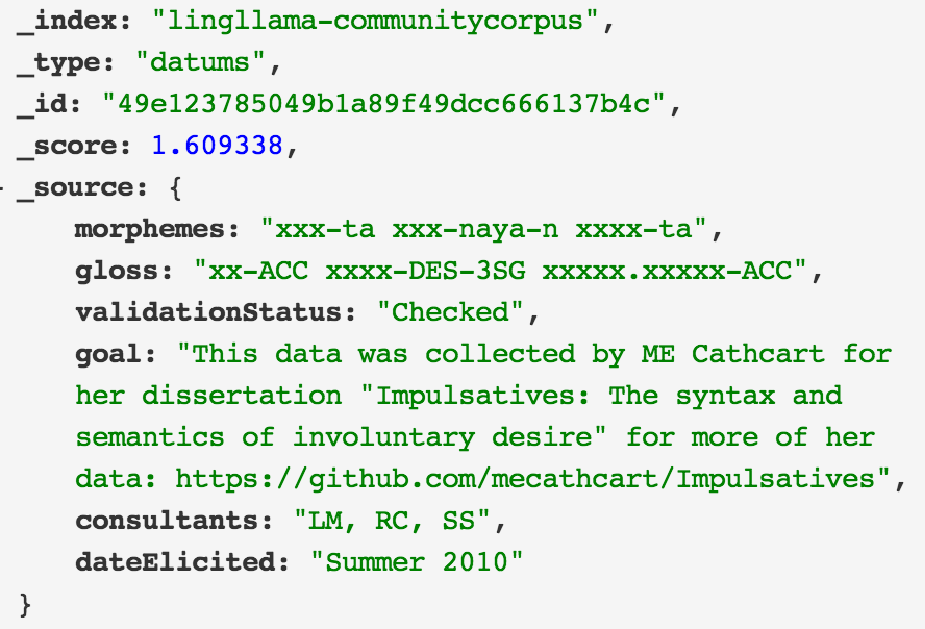
\includegraphics[width=0.4\textwidth]{confidential}

\label{ex:discoverable}
\end{exe}


\item {\bf Access}: Data is accessible. 
 
Much of linguistic data sits in researchers' offices in the form of notebooks or tapes, or as files on their computers.  LingSync data is online, and team members can even replicate the entire database (\ref{ex:accessible}) onto their laptops or department servers. Unlike tape-data and note cards, the data can be in many physical locations at one time, even available to collaborators across the world. 

\begin{exe} 
\ex a) Data can be fully replicated/accessed in its entirety

 \centering
   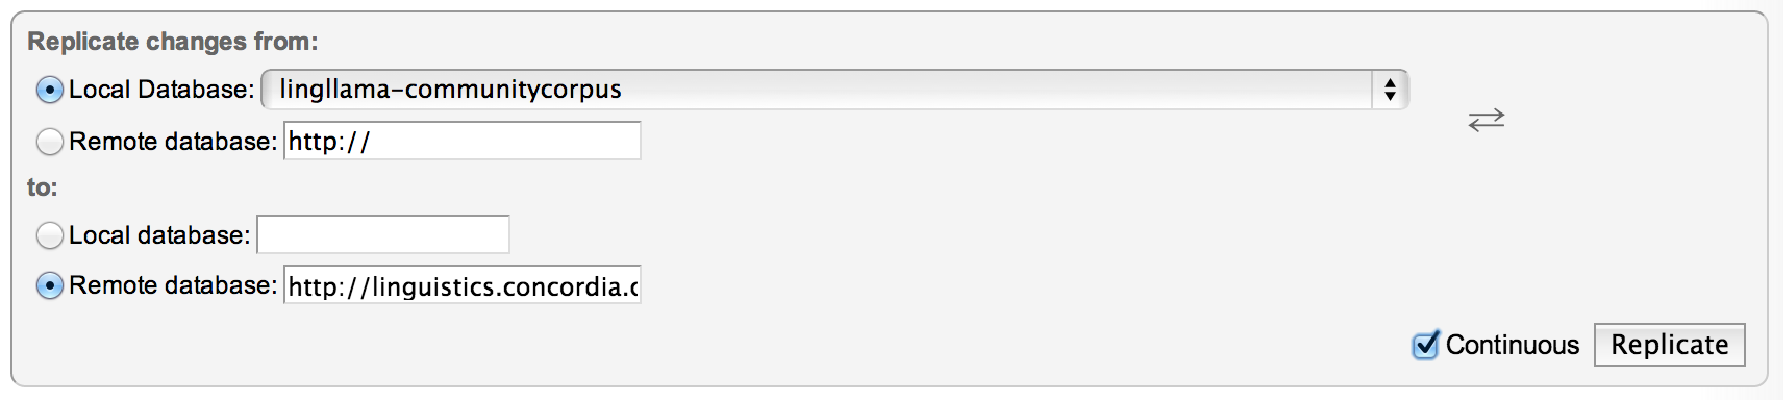
\includegraphics[width=0.8\textwidth]{accessible}

\label{ex:accessible}
\end{exe}

\item {\bf Citation}: Database provide citation information. 
 
%Providing correct and up-to-date citation information is important for online resources. Data should not be associated with obsolete or inaccessible URLs.  
In LingSync, each record  and media resource of each corpus has a unique URL (\ref{ex:discoverable}a) which can be used for citation. 
All data points are tied to an Elicitation Session which contains details of data source (such as language consultant (\ref{ex:discoverable}b), publication, or web page) and the time the data is elicited, as well as other metadata as determined by the team conventions to ensure that data quality can be traced to its source. 

\item {\bf Preservation}: Data are archived in a way that withstands long-term preservation.\footnote{http://emeld.org/school/classroom/archives/finding-archives.html}

Preservation of digital data is always confronted with the possibility that the data file format over time becomes obsolete and unsupported by new technology. LingSync stores data in a plain text JSON format  (\ref{ex:intelligible}). 
JSON files  are equivalent to XML, they are light-weight text files in which data contents are easily readable by humans and scripts. In addition to a host server, the data can be stored in multiple locations  (\ref{ex:accessible}). 
In addition, corpus administrators  can schedule regular archiving by creating a "bot" which will archive their data to one of the existing, reputable language archives of the user's choosing.\footnote{http://emeld.org/school/classroom/archives/index.html} 


\item {\bf Rights}: Rights of authors of data and of language consultants are respected. 

Each corpus includes a section for the Terms of Use (\ref{ex:customtermsOfUse}) where authors of data can specify conditions for data usage. 
Corpora often contain sensitive information, consultant stories and other information which must be kept confidential. 
%Having confidential data in plain text in a corpus forces the entire corpus to be kept confidential. 
%With LingSync, researchers and language consultants (authors of data) have control over who can see, edit and/or export which part of their data. 
In LingSync, data and information designated as confidential are encrypted prior to storage in the database using the US Federal approved AES encryption standard, and are presented as masked data (\ref{ex:discoverable}b). 
%This ensures that confidential data cannot be leaked if a corpus is shared or leaked without the consent of the corpus' author(s). 



\begin{exe} 
\ex a) Teams can have custom terms of use

 \centering
   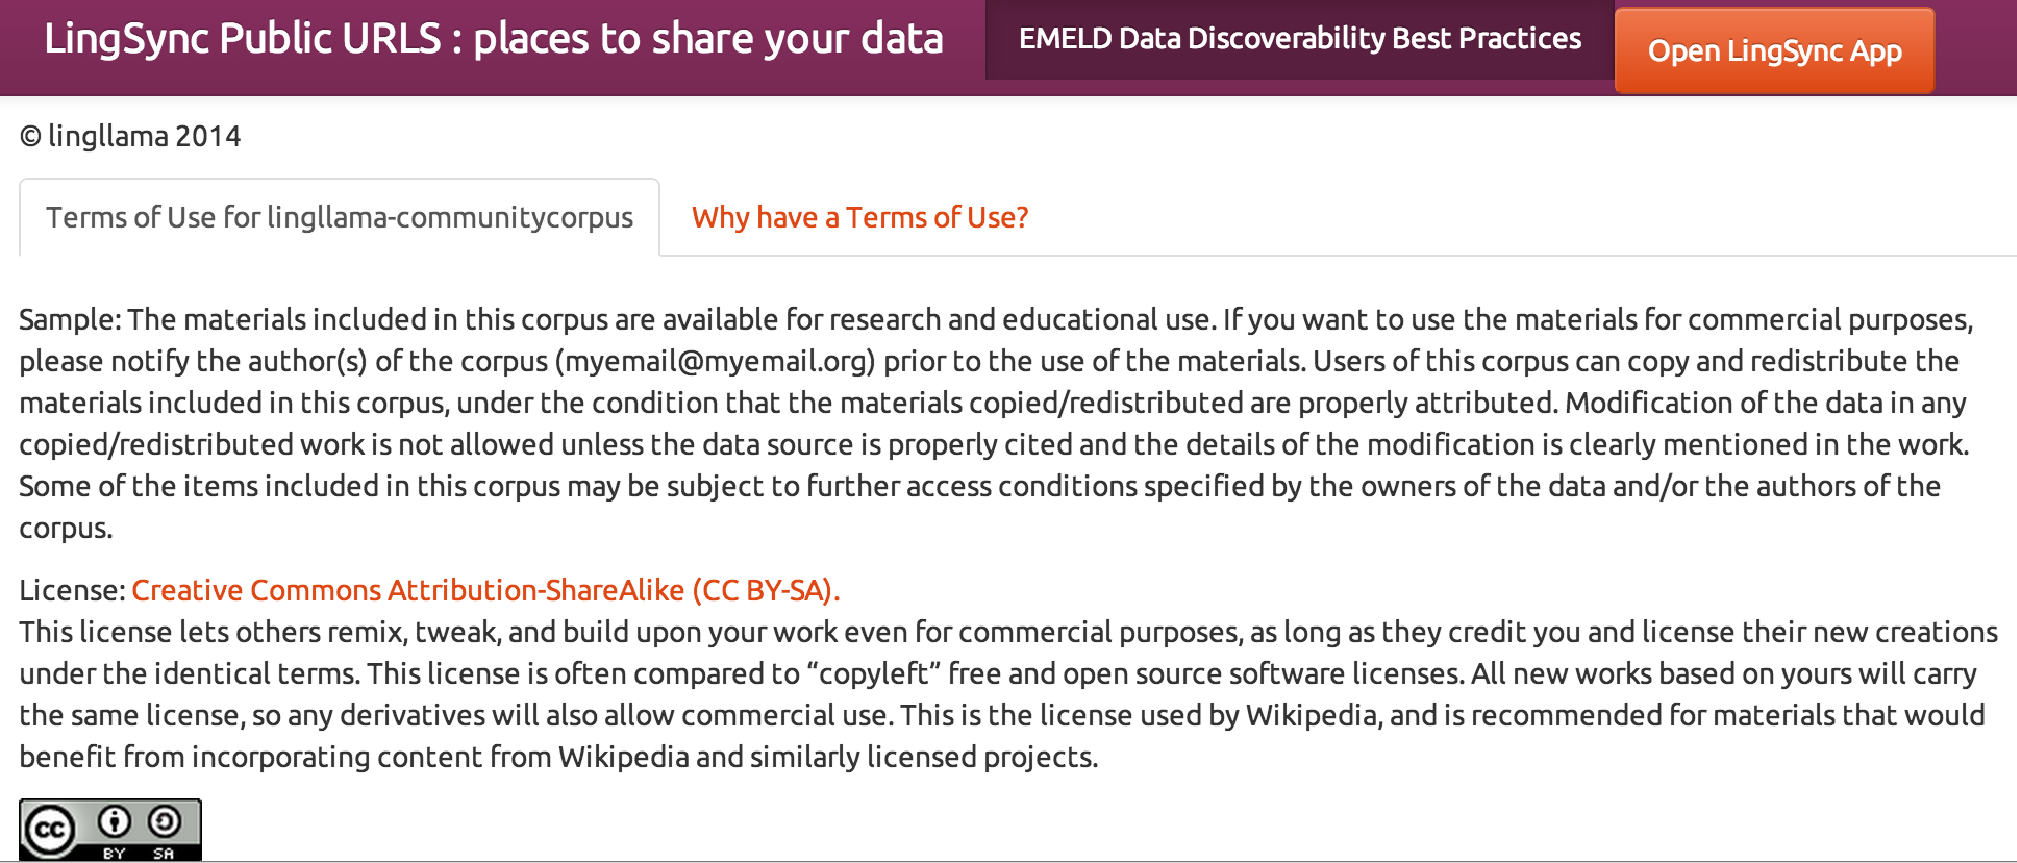
\includegraphics[width=0.8\textwidth]{customtermsOfUse}

\label{ex:customtermsOfUse}
\end{exe}

\end{description} 





\section{What is LingSync?}
\label{sec:what}

LingSync integrates the common features of existing fieldwork database software,
while addressing many of the data management practices of E-MELD and DataOne.\footnote{See the LingSync WhitePaper\\ https://github.com/OpenSourceFieldlinguistics/FieldDB/blob/master/docs/WhitePaper.pdf?raw=true}
LingSync's functionality can be divided into two groups: functionality for linguistic field databases,
and functionality for user friendly community driven software.
In this paper we will place more emphasis on the linguistic field database functionality and only gloss over some of the software engineering practices which make LingSync a usable and maintainable system. 

\subsection{Core Functionality}
\label{sec:core}
\subsubsection{Data entry and import}


Data entry in LingSync goes beyond just typing or transcribing data.
While simply typing in or importing data is the most common use case,
LingSync also provides the ability to add comments to any data in the system.
This makes it possible to collaboratively enter and discuss data,
without modifying or destroying information in the data itself.
This means that multiple team members can suggest new segmentation,
new gloss information,
or qualms about translation or context,
and the team can reach a consensus together without blocking team members from accessing or improving data.
Comments are also searchable, editable and deletable,
and can be formatted using Wiki markup which essentially permits the ability to add unlimited documentation to a data record without needing to put the documentation into the record's utterance or translation lines.
%for example.
When working as teams composed of linguists or community members who may speak different dialects,
and thus have differing judgements,
we believe that comments are a key way in which teams can provide a maximum amount of access and curation,
without worrying about different team members over-writing each other's judgements.


Since all documents in the system are versioned,
mis-guided edits by team members can be undone and detected via the team activity feeds \S \ref{sec:sharingactivityfeeds}.
If a team discovers one of its members is not following their team's data curation conventions,
the permissions system \S \ref{sec:sharingactivityfeeds} allows the team to set the individual's permissions to read and comment only.
 

Data can be categorized using tags as well as by validation status of each individual data entry.
A record could have a status as simple as "Checked," or even ''CheckedWithSeberina'' or ''ToBeCheckedWithConsultant'' (shown in example \ref{ex:consistent}. above) if the team is working with multiple consultants and/or dialects.
The ability to group data into its validation status further aids organization and permits the team to gather data for future elicitation sessions,
or to send data to consultants to be checked either by exporting the data and sending it by email,
or by adding the consultant as a team member. 

LingSync is ``skinnable,''
which means that each user can have a different visual representation of the data.
Teams can even create non-technical views of the data so that the consultants enjoy being part of the team, and feel more connected and included in  the collaborative nature of the language documentation effort.


In most teams with long standing databases,
it is often the custom to enforce conventions by providing users with drop-downs where they must select only from appropriate options,
or go to another screen to add the new option before selecting it.
\cite{Palmer:2009}, \cite{Cihlar:2008}  and \cite{Wittenburg:2006} among others state the need for tools to adapt as a field work project matures and analyses change, 
``Carletta et. al. (2000) argues that linguistic data sets are varied and idiosyncratic to the point where imposing a universal annotation/description scheme would be impractical and counterproductive''   \cite[p.11]{Cihlar:2008}. Wittenburg argues that a software's ``ergonomic qualities greatly contribute to the experience and appreciation of the every day user. Also the level of productivity that can be reached is of utmost importance.'' \citep[p.1559]{Wittenburg:2006}.
Rather than enforcing universal data conventions,
or making heavy use of drop downs, 
LingSync makes uses of  typeahead and autocomplete, 
and makes data entry and data curation also fully scriptable.
As such a fundamental part of field work is exploring and re-analyzing data,
LingSync allows users to create bots which partly automate these tasks.
Bots can even be scheduled to run periodically on the corpus (\ref{ex:bots}a),
reducing the manual data entry process if,
for example,
the team decides all data should use the convention ``ACC should be glossed as CAUS in the context of ASP.'' Bots are able to go through a corpus,
and leave comments on data which should be cleaned manually,
or even execute the changes (\ref{ex:bots}b) after the team has reviewed and approved the changes.
%There are existing bots for transliteration (conversion of Inuktitut syllabics to romanization) and for duplicating morphemes fields to allomorphs fields,
%among others.
%Bots are provided to help reduce the repetitive tasks,
%freeing team members to focus on data entry and data analysis.


%We believe strongly, as do the creators of  ELAN that 
%Rather than place the weight of data validation at the time of data entry, typeahead suggestions (\ref{ex:consistent}) are provided to encourage team members to use existing annotations, 
%% fields can be populated with autocomplete lists which display options ,
%but still permit new options to be added without visiting an additional screen. 
%Bots allow the validation to happen after data entry by identifying context to be combined or separated, and even in some cases executing the cleaning automatically.


\begin{exe} 
\ex Bots/Scripts can be scheduled to verify data consistency

\hspace{-1in}
 \centering
   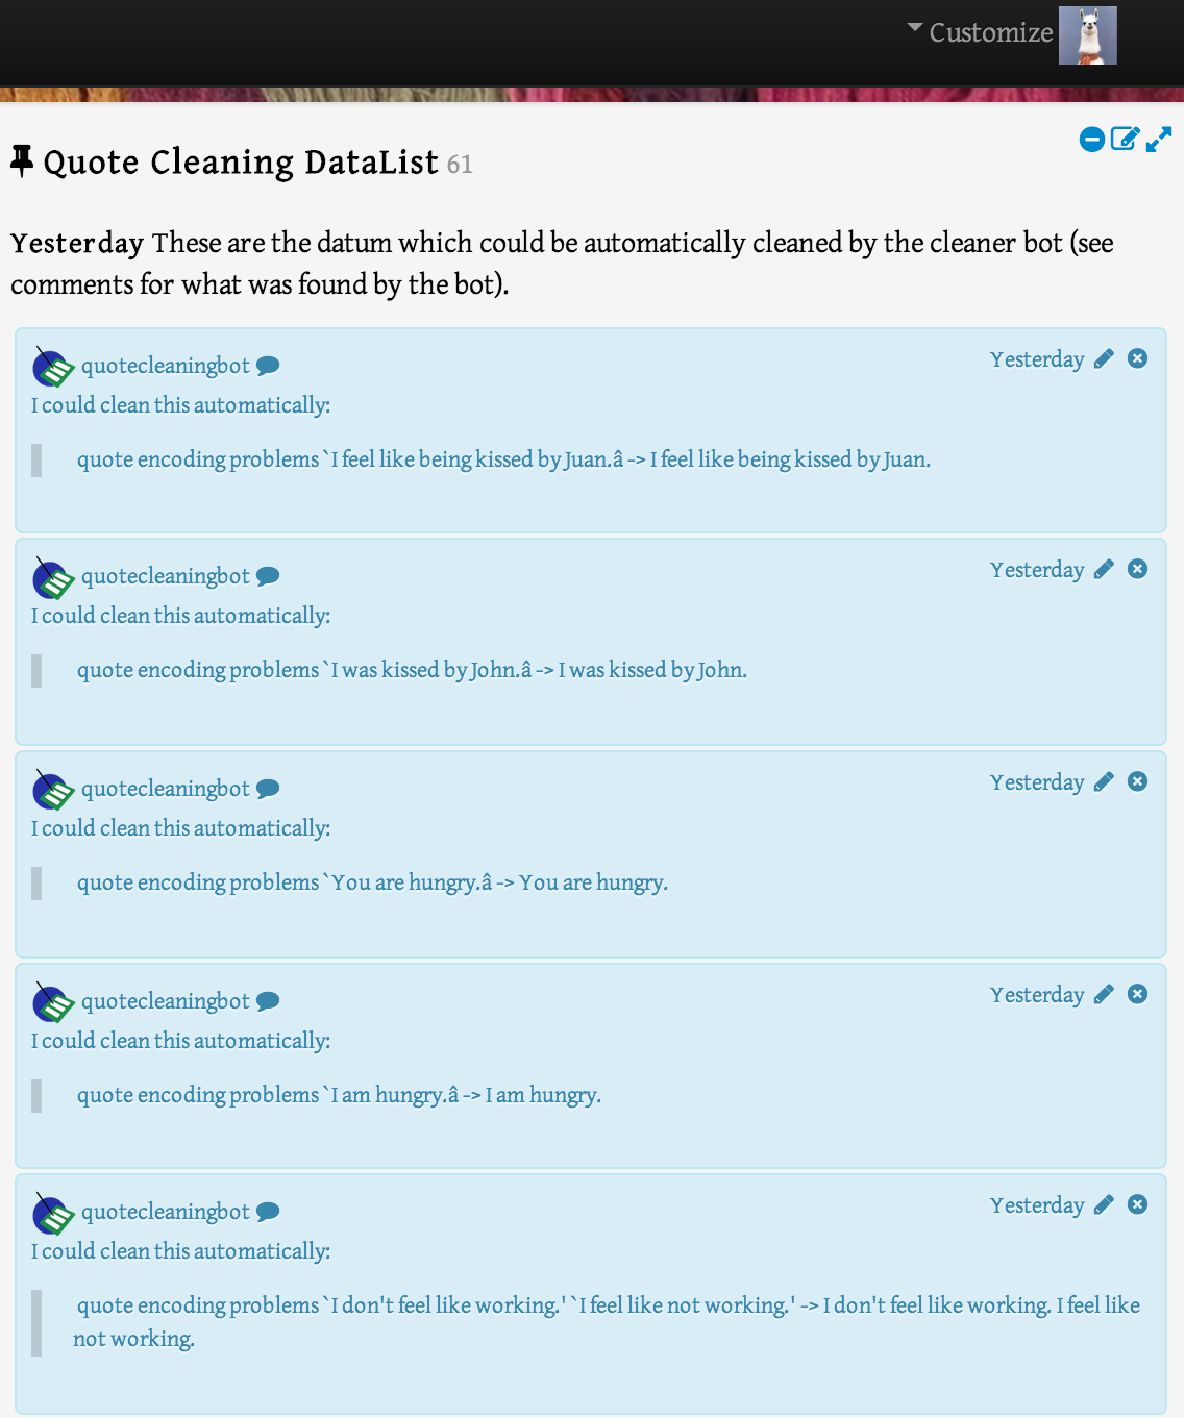
\includegraphics[width=0.45\textwidth]{cleaningBotsDatalist} ~
   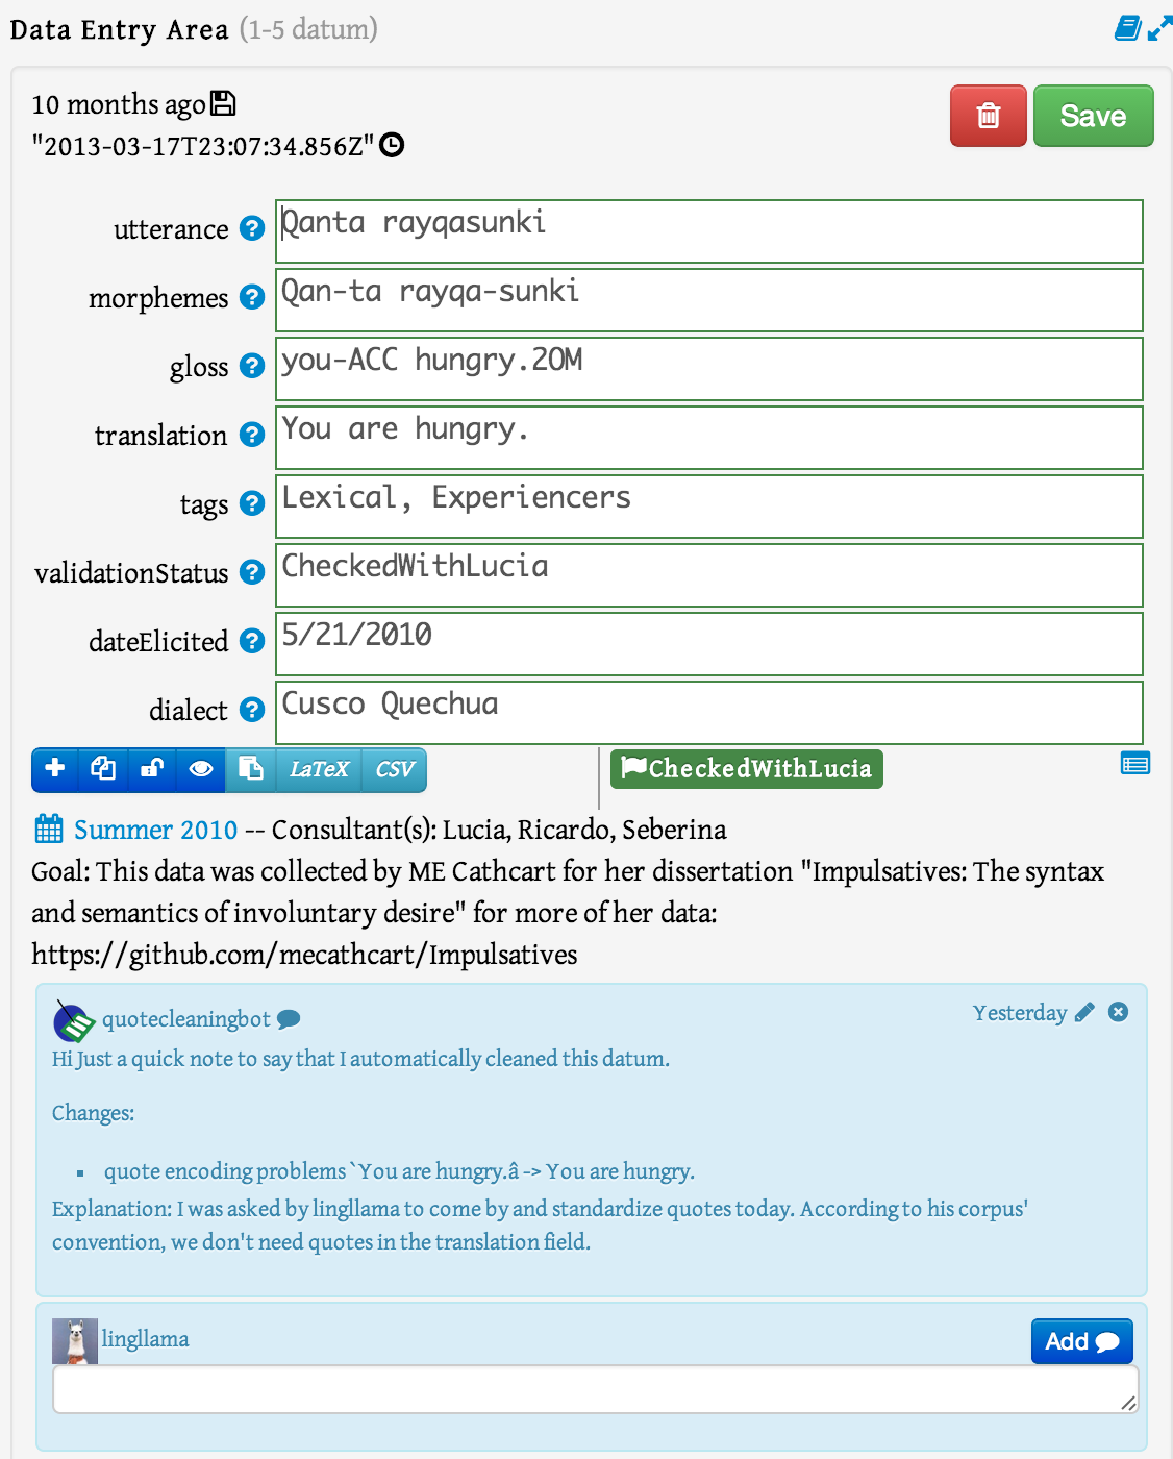
\includegraphics[width=0.45\textwidth]{cleaningBotCameBy}

\label{ex:bots}
\end{exe}



Data entry is expected to be grouped by elicitation session (or by publication or other data sources).
In fact,
one expected method of data entry is not data entry at all,
but rather the video recording of an elicitation session followed by typing up the session at a later date.
Longer audio/video files can also optionally be uploaded to the speech web service \S \ref{sec:phoneticwebservice} to be automatically split into utterances,
 reducing data entry and record creation if a team wishes to record elicitation sessions and enter the data later.
 This approach to data entry permits the team to dedicate 100\% of their attention to the speaker and formulating questions while eliciting data,
rather than dividing their attention between the speaker and the process of data entry.

One of LingSync's founding principles is that you should only need to enter data once.
Whether you enter it in an Excel Spreadsheet,
in a handout,
in ELAN or in FLEx,
you should be able to import it into LingSync without needing to re-enter the data.
 Each record in a LingSync database can have an unlimited number of fields,
with unlimited complexity,
making it possible to import other formats,
and be able to re-export them without losing any information (for example,
timed alignments in ELAN or Praat).



\subsubsection{Auto-glosser}

 

Similar to the glosser underlying FLEx \citep{Black:2006}, the semi-automatic glosser requires no configuration or set up to be useful.
It ``learns'' from the data in a corpus to guess where morphemes might be segmented (\ref{ex:glosser}a),
or how morphemes should be glossed.
The glosser is also a separate module,
which means that if you have an existing glosser, you can plug it in to LingSync.
Glossers can also be shared.
For example,
if you have two Quechua corpora,
you can set the glosser URL to use either corpus, or permit other teams to use a glosser which was trained on your corpus.
 


\begin{exe} 
\ex The glosser offers a) morpheme segmentation using b) precedence relations in your corpus

 \centering
   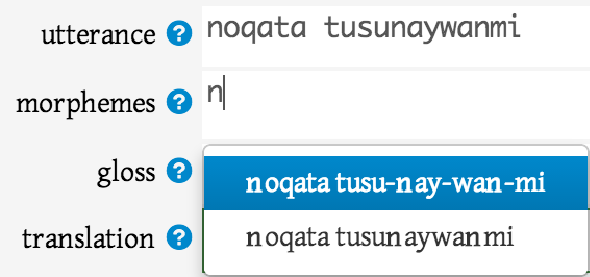
\includegraphics[width=0.45\textwidth]{glosser} ~
   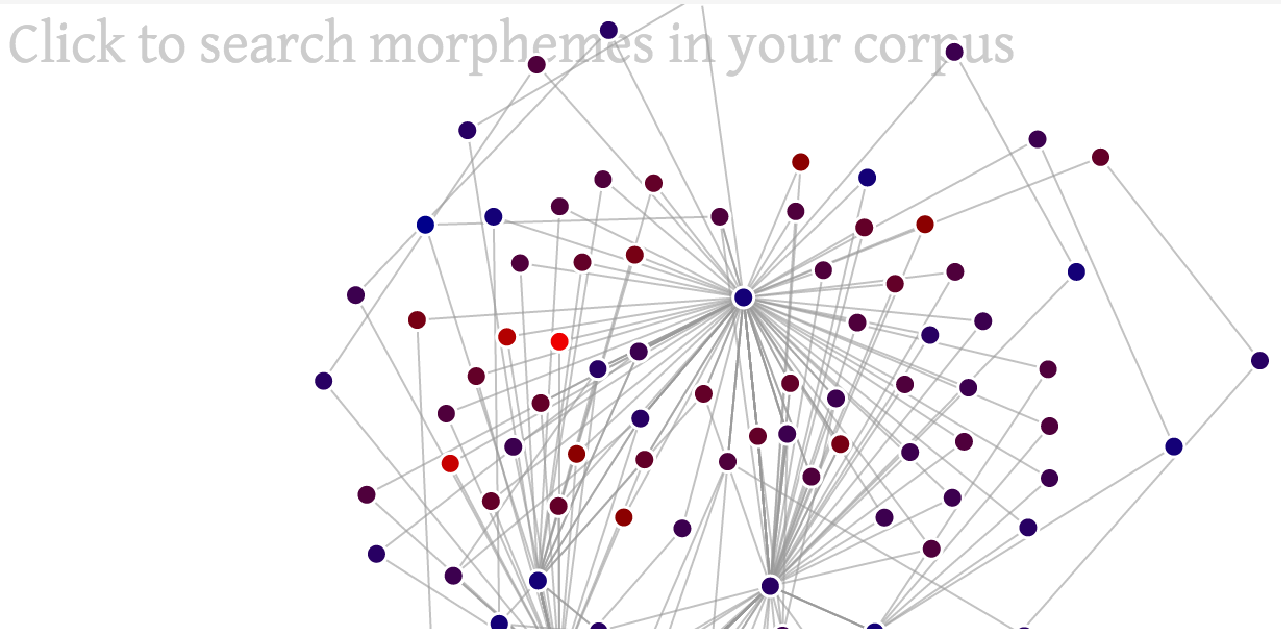
\includegraphics[width=0.45\textwidth]{morphemePrecedenceRelations}

\label{ex:glosser}
\end{exe}


The glosser is designed to make the app ``smarter'' and to reduce the amount of time spent entering predictable information such as glosses.
The glosser can use any existing morphological analysis tool (\S \ref{sec:plugins}) to break down the utterance/orthography line  into a probable morphological segmentation using known morphemes in the lexicon,
and enters a probable gloss for the morphemes in the glossing line.
The glosser module is designed to reduce redundant data entry,
not to provide complete glosses.
It is of course crucial that predicted morpheme segmentation and glosses be corrected by users,
particularly in languages that have many short or ambiguous morphemes,
which will result in more possibility for error in automatic morpheme segmentation.
 

The glosser uses the auto-generated lexicon to evaluate morphemes both by precedence relation and by gloss.
Each corpus has its own lexicon,
which is loosely modelled after a mental lexicon,\footnote{It is important that note that LingSync uses a lexicon, not a dictionary. The lexicon is a connected graph similar to theoretical models of mental lexicons, and is useful for linguistic analysis but not useful for producing a dictionary for a language community. LingSync is not suitable for curating dictionaries and the tasks involved in professional lexicography. Instead LingSync offers export to WeSay which makes it possible to build a community driven living dictionary. http://www.sil.org/resources/software_fonts/wesay} 
as a network of morphemes,
allomorphs,
orthographie(s),
glosses and translations.
% % (for a dictionary see the Dictionary plugin in \S~\ref{sec:plugins}).
%As a connected graph (\ref{ex:glosser}b) it is the most useful structure to index datum and search for datum real time while data entry is happening.


\subsubsection{Search}

LingSync was designed for powerful search.
Users can search a corpus (\ref{ex:searchable}),
or across multiple corpora (\ref{ex:discoverable}).
Similar to ELAN \citep{Wittenburg:2006}, 
the results of  searches can even be saved as Data Lists which can be sorted and
saved for later exporting, curating for a handout or curating for language learning lesson for heritage speakers.

Search can be as simple as a keyword search,
which will search the entire record,
or search within only one field,
or for example one key word in one field or another key word in another field.
For those users who like to think in Set Theory, LingSync provides the ability to look at the Intersection or the Union of search results. 
For phonologists, LingSync allows search using regular expressions to find segments in context.
If there is demand, we can add the ability to search for minimal pairs or to search for phonological features in context using a phonology ontology (a general purpose feature geometry/articulatory feature ontology,
or a customized ontology created by the users for their language of interest)  where feature geometry searches could be used.
Phonological search can also be helpful in %search for potential minimal pairs or phonological features in context to verify with consultants,
preparing stimuli and controlling confounds for psycholinguistic experiments.


\subsubsection{Sharing corpora,
activity feed}
\label{sec:sharingactivityfeeds}

Sharing primary resources and the inconstant results of field work is notoriously difficult, 
``most linguists fail to share their data for reasons ranging from the difficulties involves in curating it into a distributable form, to concerns regarding speaker privacy, to a desire to be finished working with it on their own before giving others access'' \citep{Bender:2010}. Even ``a funding body like the ELDP cannot get all of its grantees to deposit in an archive in a timely fashion (or at all)'' \citep{Thieberger:2012}. We hope to make this process easier  for teams by importing any format, letting users write scripts to clean data, mark some or most data as confidential or not-yet-verified, to help get the data into a state where the teams can publish it to a long term archival organization such as OLAC or the original granting agency. Part of the process of preparing data for publication involves collaboration of what data needs to be cleaned or excluded.


Corpora in LingSync can be shared as a team,
with administrators,
who cannot see the data
but can add new team members (e.g.
a project coordinator); writers,
who cannot read the data but can enter new data (e.g.
language consultants,
or psycho-linguistic experiment participants); readers,
who can see the data but cannot edit it (e.g.
external collaborators) and commenters,
 who cannot edit the data but can provide feedback and offer additional information or corrections (e.g.
consultants and/or collaborators).
 Of course,
most teams will choose to give all roles to all users,
but these roles permit a wider and inclusive data collection team than previously available  in other data management tools where the permissions are simply full access or no access.

As a team,
users might also want to catch up on recent activity in the corpus.
If the corpus is small (only a 100 records) users could simply read each record to see what is new,
but for larger corpora or where there is more activity, LingSync provides team activity feeds.
In the activity feed widget (\ref{ex:activityfeeds}) users can see who has modified,
commented and
created data,
as well as recorded/uploaded audio,
or put records in the trash to be deleted later.
There are also user activity feeds which are only presented to the user. %Although less interesting than the actions of one's teammates,
A users' personal feed  can help them remember what they were working on last time,
particularly if it has been months since they last opened the corpus.
%We expect users will visit their corpus very frequently
%when building it,
% but visit only sporadically as they need to return only to consult their data.
For example,
the user activity feed could help you remember that you hadn't finished typing up that elicitation session three months ago before you had to go to class.
``We all know of projects which have been completed and for which there are now large datasets that are not being properly maintained.''\citep[p.133]{Thieberger:2012} By introducing activity feeds as a feature of a field linguistics database, we hope that teams will return to their data, and continue to curate it even after they have created their handouts, given talks and moved on to other aspects of their research. 

\begin{exe} 
\ex Activity feeds let team members catch up on recent changes in the database

 \centering
   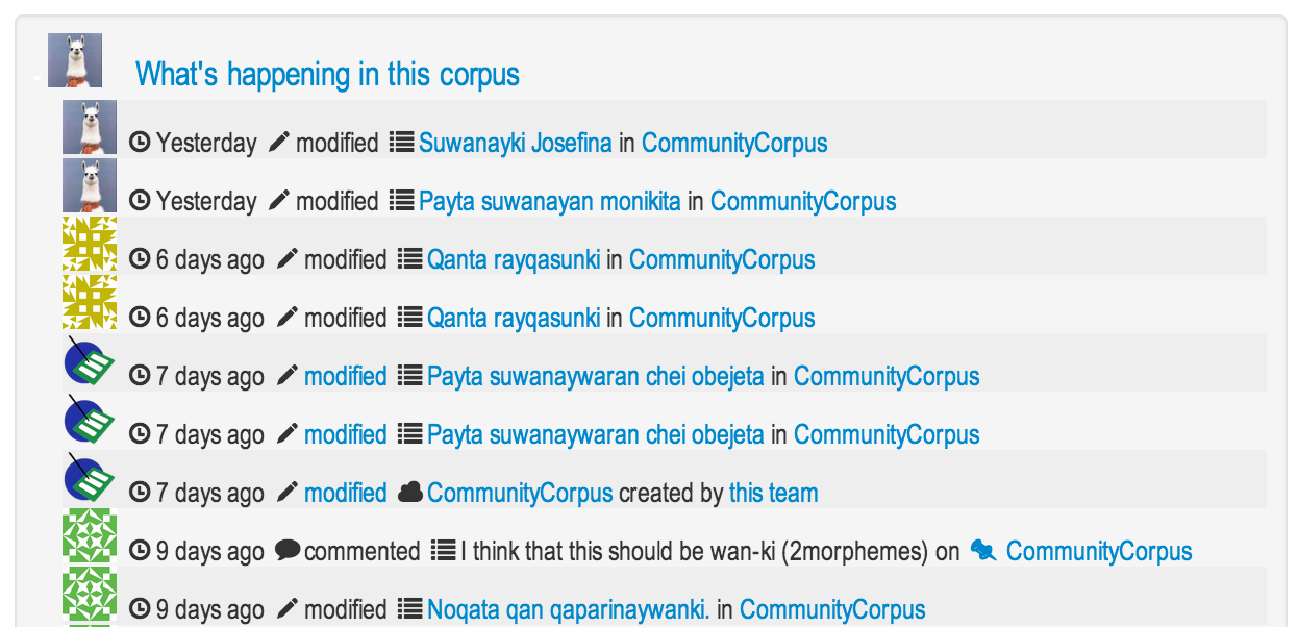
\includegraphics[width=0.7\textwidth]{activityfeeds} 

\label{ex:activityfeeds}
\end{exe}

\cite{Thieberger:2012}  identifies two ways in which research must be shared, with a unique URL so that researchers are able to cite primary resources, which further permits ``combining data from disparate sources (which could be `mashups' or could, for example, involving correlating transcripts and media in `compound objects').'' LingSync addresses both concerns by a fine grained level of sharing where the user controls what is shared and how, while each resource keeps a unique URL.\footnote{ \cite{Musgrave:2012} discusses the diverse ways a language community can benefit from language documentation and how different communities benefit differently. LingSync's sharing system permits prototyping `mashups' early in a collaboration that can result in data collection which suits not only language documentation efforts but also the needs of  unique language communities.} 
Corpora can also be shared via export in EOPAS XML format and import to EOPAS.org.

%Encouraging a unified terms of use across corpora permits better integrability of corpora among researcher groups,
%as well as the creation of mobile apps and content dissemination networks for heritage speakers and members of the language community diaspora.
%Like EOPAS \citep{EOPAS:2014:Online} LingSync encourages all teams to adopt a Creative Commons license for their resources,
%however, each LingSync corpus team can choose to have its own terms of use (\ref{ex:customtermsOfUse}) and licensing which permits the maximum flexibility to teams.
%Embeddable widgets and unique URLs to data can be shared.




%\subsubsection{Custom settings}
%
%LingSync is highly customizable.
%It comes with the ability to choose from 5 dashboards,
%and allows users to even create their own.
%Users can decide how many records to show on a page of data,
%in which order the records to be shown, for example. % and many more options.
%For users who have limited eyesight or who are using screen readers,
%LingSync provides a high-contrast option as well as a dark option to reduce eyestrain after hours of entering data.
%LingSync was designed partly by research assistants who had entered data for 40 hours a week,
%and so it also provides the ability for rich and  interesting background pictures to keep entering data visually stimulating.
%
%Each corpus is also fully customizable: team members can add new fields to the corpus,
%as well as edit its terms of use and other information which can become important if the team decides to share the result of their work with the outside world.
%Customization is a pervasive aspect of LingSync and has affected the way each functionality was conceived and implemented.


\subsubsection{Export}

As users of many diverse data management software,
we felt it was crucial that LingSync be non-proprietary and open. In a language documentation project,  linguistic data must remain usable even when ``the delivery system (which could be proprietary software or websites that are no longer maintained) becomes unusable'' \citep[p.132]{Thieberger:2012}.
One important aspect of this is the ability for teams to export their database in any format they choose,
in its entirety, or only portions of data which are relevant to a certain export goal.
Teams can even save lists of data for dedicated export purposes,
such as data for a handout,
or data which they are curating to be published as stories for the language community they are working with.
LingSync is also able to export word lists,
which can be used either as language learning exercises for heritage speakers or as materials for field methods courses.
\cite{Thieberger:2012} points out that ``offline use is likely to be most relevant to speakers of the languages recorded, given the lack of affordable -- or indeed any-- internet access. Such offline use of language records includes printed outputs and media on CD, DVD, or in computer-based (e.g. iTunes) formats.'' 
It is possible to export an entire corpus either as a ZIP archive,
as well as multiple formats such as XML, JSON, plain text, TextGrid, LaTeX  and CSV.\footnote{Currently there are no users using ELAN which we know of, so export to ELAN is not currently available.} Like the Washo Project, LingSync seeks ``a format that is `self-documenting' so that it will be usable years after when the current technologies used to manipulate the data have long become obsolete'' \citep[p.4]{Cihlar:2008}. When data is exported in its raw form, each field includes the help conventions which were used in the app by teams to tell each other what the field is for. When corpora are exported as a ZIP archive, these help conventions are used to automatically generate a README file which details the corpora's fields as recommended by E-MELD \S \ref{sec:design}.

Beyond export,
LingSync databases are fully replicable between servers (\ref{ex:accessible}),
which means that team members can have entire copies of their database locally on their laptops,
while still remain in full sync with other team members when they go online.
It also means that organizations can back-up their data to their own servers without worrying that data may become stale or out of date.




\subsection{Plugging into LingSync}
\label{sec:plugins}


One of the strengths of LingSync is that it is built using well-understood web technologies which permit the creation and integration of nearly any existing software as web services. 
Even complex user interfaces can be combined and integrated with LingSync via the NPM and Bower web module management system.\footnote{
For teams collaborating with Computer Science or Software Engineering departments, there are limitless plugins which port advances in Computational Linguistics  and Natural Language Processing libraries  \citep{Chen:2011}  including as negation and modality scope taggers for  GATE \citep{Cunningham:2011} NLP pipelines based on  \citep{Rosenberg:2012} or mobile apps which take advantage of diverse NLP pipelines wrapped in web services \citep{Sateli:2013},
 handwriting recognition research for low resource languages \citep{Sadri:2007} or even training for speech recognition systems with as little as one hour of annotated data using web-services which wrap open source toolkits such as Sphinx-4 \citep{Walker:2004} or Kaldi \citep{Povey:2011}.
Sample web services are provided on the OpenSourceFieldlinguistics GitHub.\footnote{https://github.com/OpenSourceFieldlinguistics} %\citep{Desilets:2010}
In this section we will discuss only a few of the current web services.}

\subsubsection{Custom glosser}

 Benoit Farley's \citep{Farley:2014:Online} morphological analyzer for Inuktitut was wrapped into a web service using Node.js, permitting a glosser which was prepared to look up variant  surface realizations of morphemes in Inuktitut corpora.

\subsubsection{Language learning module for Android}

A prototype mobile app for language learning was build which  enables researchers and language teachers to create language learning aids from the data in existing corpora and from the data newly collected for the purpose of language learning.
The language learning prototype aims to help heritage language learners include their language as part of their daily activities and improve their listening and speaking skills.
The orthographic lines (i.e.
utterance and morpheme lines) and the attached audio or video recordings of a datum are taken as materials to create lessons. Users are also able to make their own lessons and share them with other learners.

\begin{exe} 
\ex The Language Learning prototype is downloadable on Google Play\footnote{https://play.google.com/store/apps/details?id=com.github.opensourcefieldlinguistics.android.lessons}

 \centering
   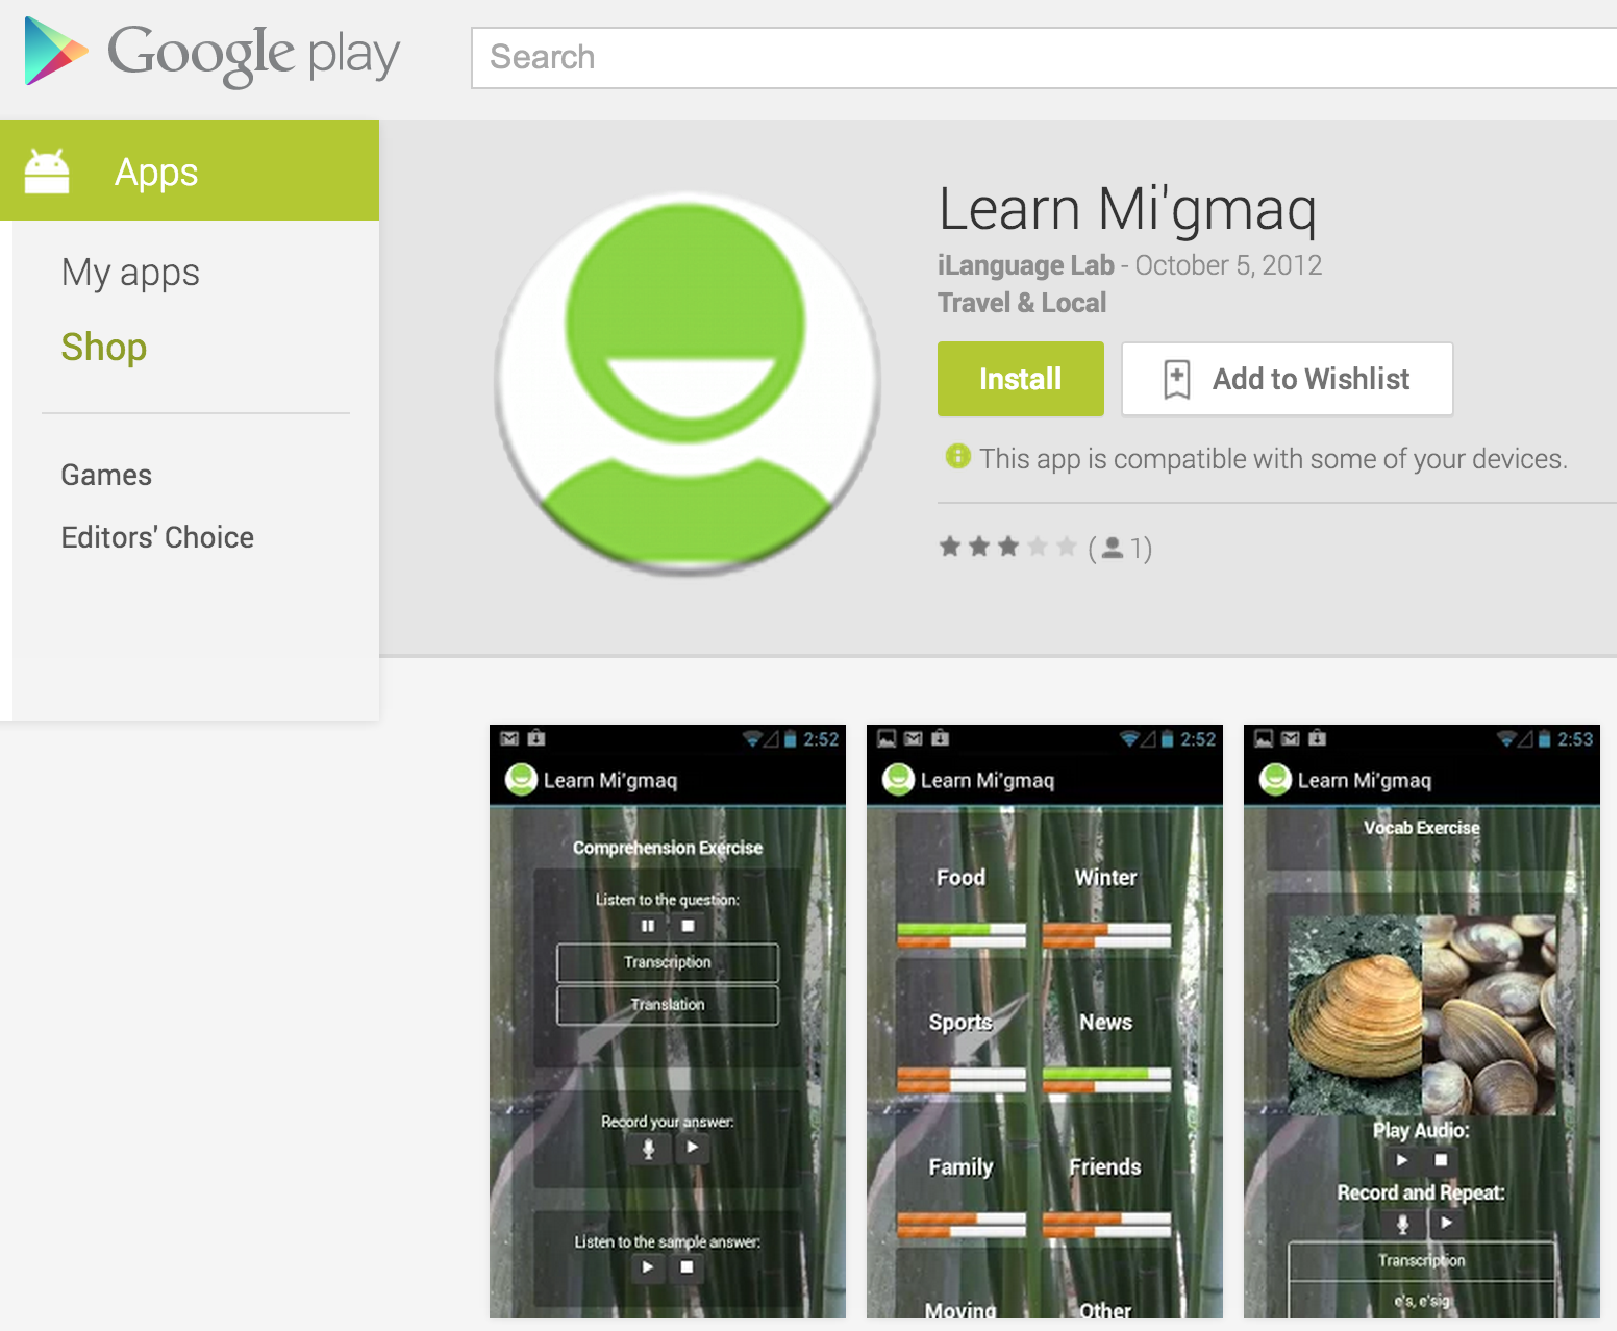
\includegraphics[width=0.5\textwidth]{languageLearningApp} 

\label{ex:languageLearningApp}
\end{exe}

\subsubsection{Integration with ProsodyLab aligner and touch tablets}
\label{sec:phoneticwebservice}

The phonetic aligner web service makes it possible to upload audio or video recordings and the orthographic/utterance lines of datum to create a dictionary unique to the language of the corpus,
and to run the McGill ProsodyLab Aligner,
a machine learning algorithm which uses Hidden Markov Models to predict boundaries between phones and creates a Praat TextGrid with estimated phone boundaries,
saving hours of boundary tagging.


We also created an Android Elicitation app which permits recording of high quality video on 7 inch or 10 inch tablets during elicitation sessions.
Multiple videos can be associated to a session and uploaded to the ProsodyLab Aligner web service for automatic generation of aligned TextGrids. 




\subsubsection{WebSpider}

The Multilingual Corpora Extractor is a type of web spider which allows teams with limited access to consultants to gather data using blogs or forums or online translations of the bible.
The web spider also provides an additional source of context to assist consultants in providing grammaticality judgements,
as well as additional contexts where morphemes appear.
For example,
``ke'' is largely considered a postposition by Urdu consultants with explicit knowledge,
however it is often produced as other functional morphemes in everyday spoken contexts.
Blog/forum data can be used to discover these additional contexts.\footnote{
If users identify a resource which needs discourse analysis, \cite{Dubuc:2010} could also be followed to create novel spiders which extract discourse structure out of social media in low resource languages.}

\section{How is LingSync used so far?} 
\label{sec:use}
%\subsection{McGill-Listuguj partnership}

%LingSync is currently in use by the Mi'gmaq Research Partnership,
%a collaborative project by McGill linguists and Mi'gmaq speakers and learners in Listuguj,
%Quebec.
%Several members of the team working with the language have been entering language data into a shared corpus since Fall 2012.

%\subsection{Field methods classes} 

LingSync was used by two field methods classes in Winter 2013,
at the University of Ottawa (Teenek) and Pomona College  (Igikuria) and is being used by three field methods classes in Winter 2014,
at McGill University (Inuktitut),
Yale University (Quechua),
and the University of Connecticut (Nepali).
The languages of these classes are typologically diverse and the teaching styles are varied.
The students and instructors of these classes have provided invaluable feedback which was used to further improve LingSync.


%\subsection{Other users} 

There are over 300 people who have created user accounts with LingSync,
all of whom together have created over 1000 corpora.
Over 150 of these user accounts are field methods students, the remaining are appear to be `investigating' accounts to try out the app.
We estimate between 10-20 teams (consisting of 1--20 users) have moved beyond the investigation phase and have been using LingSync actively.

\section{Conclusion } 
\label{sec:conclusion}

In this paper we have discussed some of the challenges inherent in field work projects. 
We argue that many of the challenges were mutually exclusive and not reconcilable in a single data management system prior to 2012. 
We have surveyed how some teams have managed to find ways to collaboratively build high quality data archives while balancing  their limited resources for research and language documentation, often in collaboration with technical consultants or Computer Science departments. 
We have presented LingSync, an open source, open ended system which helps make it easier for field work teams to focus more on data analysis,  and less on  conversion of data and other repetitive task inherent in managing an evolving data heavy project. 
LingSync was designed from the ground up to be both easy for new users to use, but also respect data management best practices. In the process, LingSync's open development and use of a unified, easy-to-learn scripting language for user interfaces, web services and data queries has empowered field linguistics labs to learn more about data automation and build internal technical knowledge, which further permits  the freedom for teams to develop novel ways of understanding and exploring their data. %explain the subtleties of language data to database administrators.

%,helping to bridge members of the technical community with the research community.

%What doesn't lingsync do: it doesnt make traditional single language dictionaries, for this communities should use WeSay, it doesnt let users transcibe speech or gestures, for this use Elan or Praat. LingSync can be used to build collocation and illustrative dictionaries, but traditional lexicography is far far more data curation than the type of data curation which goes into field work thus teams who have promissed to create a dictionary should either allocate resources to lexicography, or reevaluate whether the langauge community would be best served with a dictionary or rather with a content site that integrates with social media and can help heritage speakers interact and share content in their minority languages. 

%\label{sec:intro}

\custombib{\bibliography{caml2012}}


\end{document}


\appendix

\section{Why now: Advances in Database and Web Technologies}
\label{appendix:technology}

Since early 2010, the term \emph{NoSQL} has lead technology news. Databases can be grouped in roughly two categories, table-like (\ref{ex:whynosql}a) (also referred to as \emph{Relational}, or \emph{SQL} databases) and document-like (\ref{ex:whynosql}b) (commonly referenced in language documentation literature  simply as \emph{XML}, and in the software industry as \emph{NoSQL}).\footnote{NoSQL is actually a broad category encompasing anything which is not SQL, including documents but also interconnected web/neuron-like data strutures.} NoSQL data stores, including simple file based systems, have always existed and in fact pre-date SQL databases. Much like field linguists and language documentation standard bodies, companies who need  scalable data management such as Google \citep{Dean:2004, Dean:2008}  Adobe \citep{Lehene:2010:Online} Facebook \citep{Borthakur:2011}  and LinkedIn \citep{Sumbaly:2013} actively resist SQL (frequently proprietary) data storage solutions  (\ref{ex:databasetrends}a) and seek open source NoSQL solutions (\ref{ex:databasetrends}b). 

By April 2012 when LingSync began, NoSQL databases had matured to the extent that they were well understood, and deployed at large scale. 
Using an existing mature NoSQL database solution has greatly reduced the novel code needed to build LingSync, meaning we were able to focus our efforts on building usable user interfaces, and integrating our favourite field linguistics tools as modules and plugins to help automate the data entry process. 




\begin{exe}

  \ex   Illustration of the storage requirements vs self-documenting ability of NoSQL
  \centering
    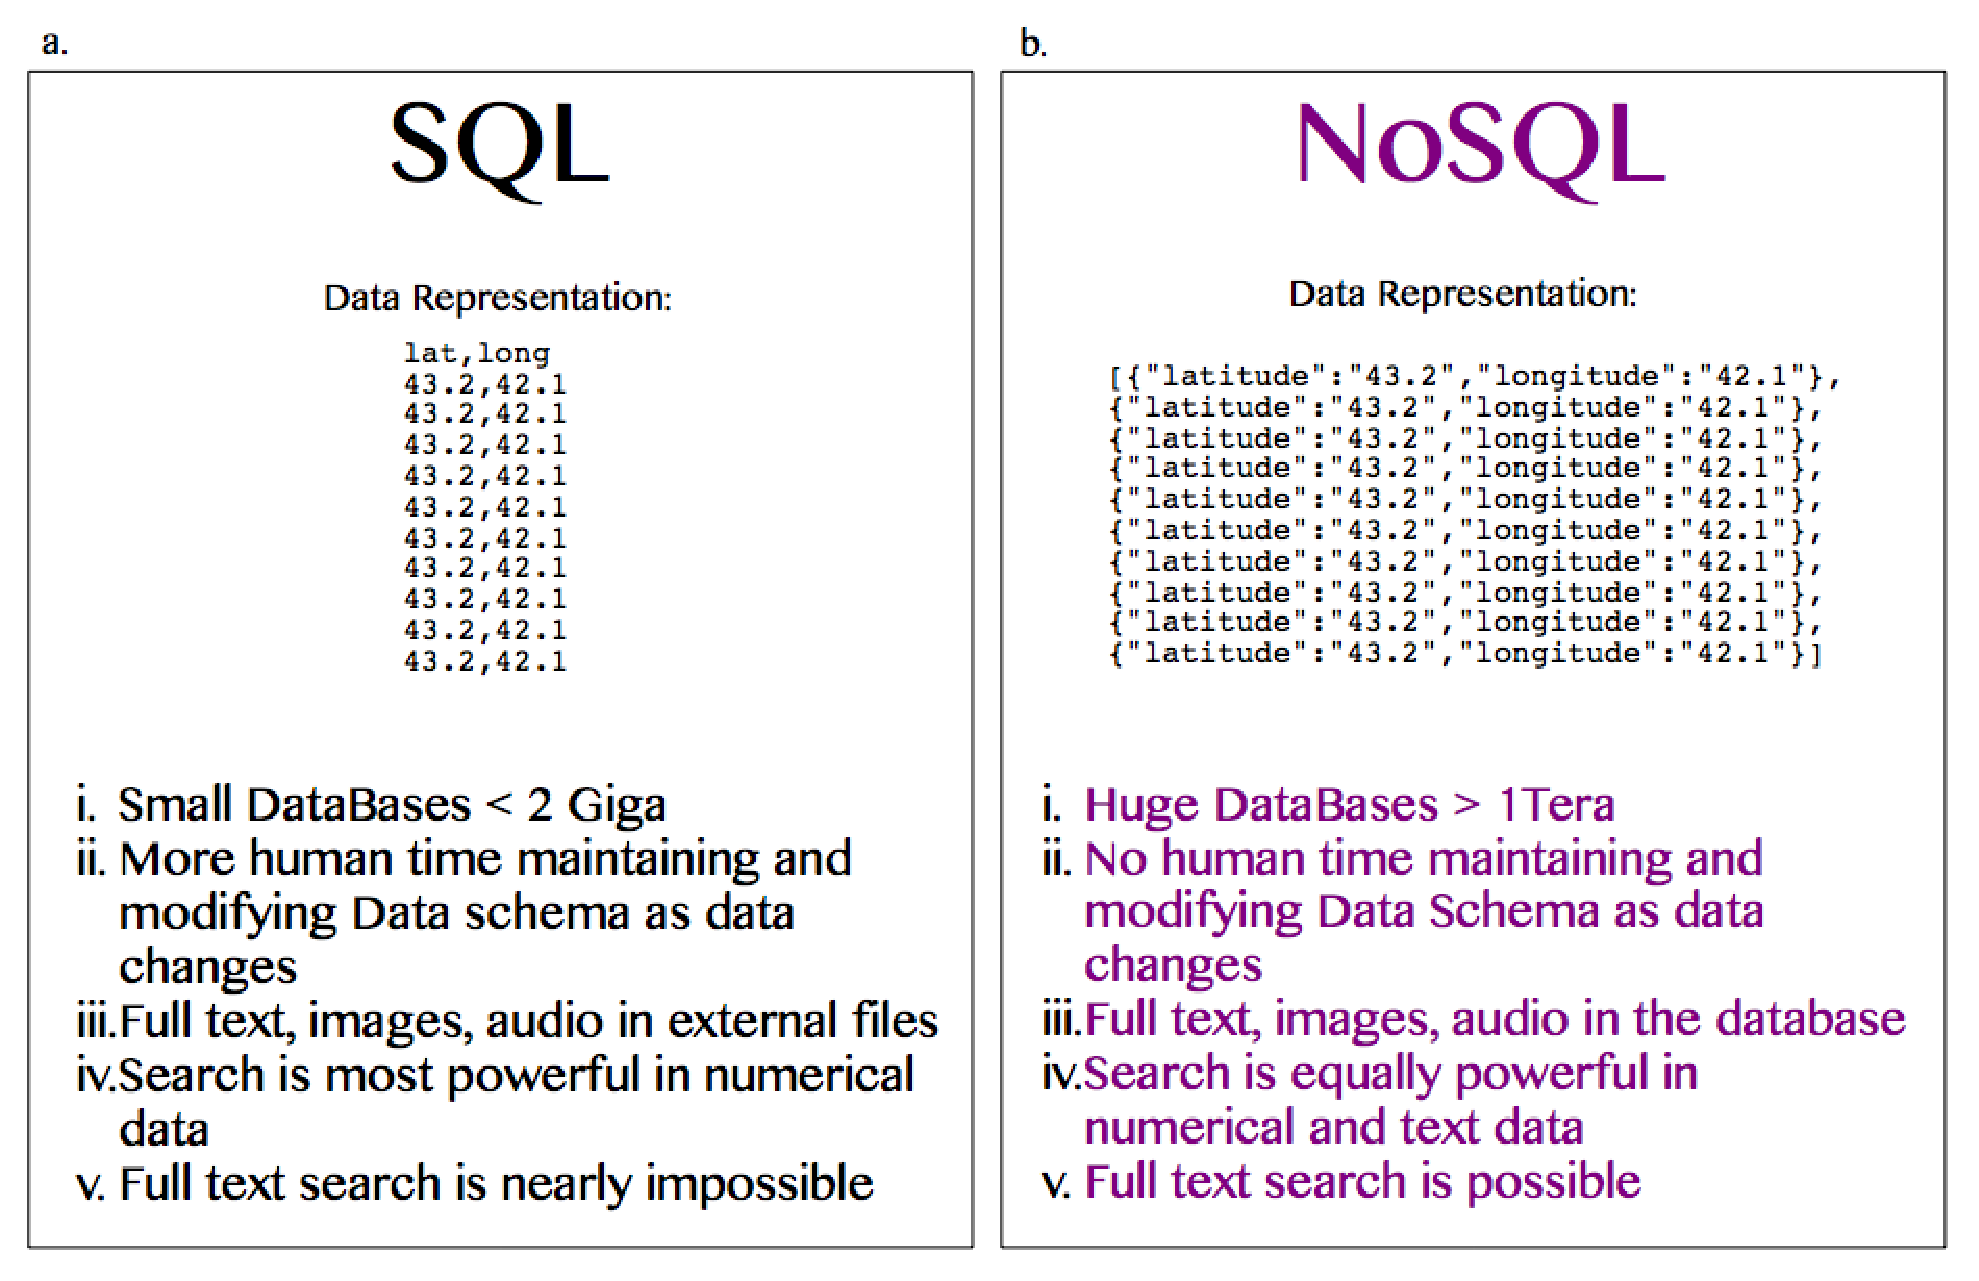
\includegraphics[width=0.8\textwidth]{whynosql}

\label{ex:whynosql}
\end{exe}


\begin{exe}

  \ex   Currently human resources are very expensive while hardware is inexpensive, resulting in a growing popularity of NoSQL databases including what is under LingSync (CouchDB)
  \centering
    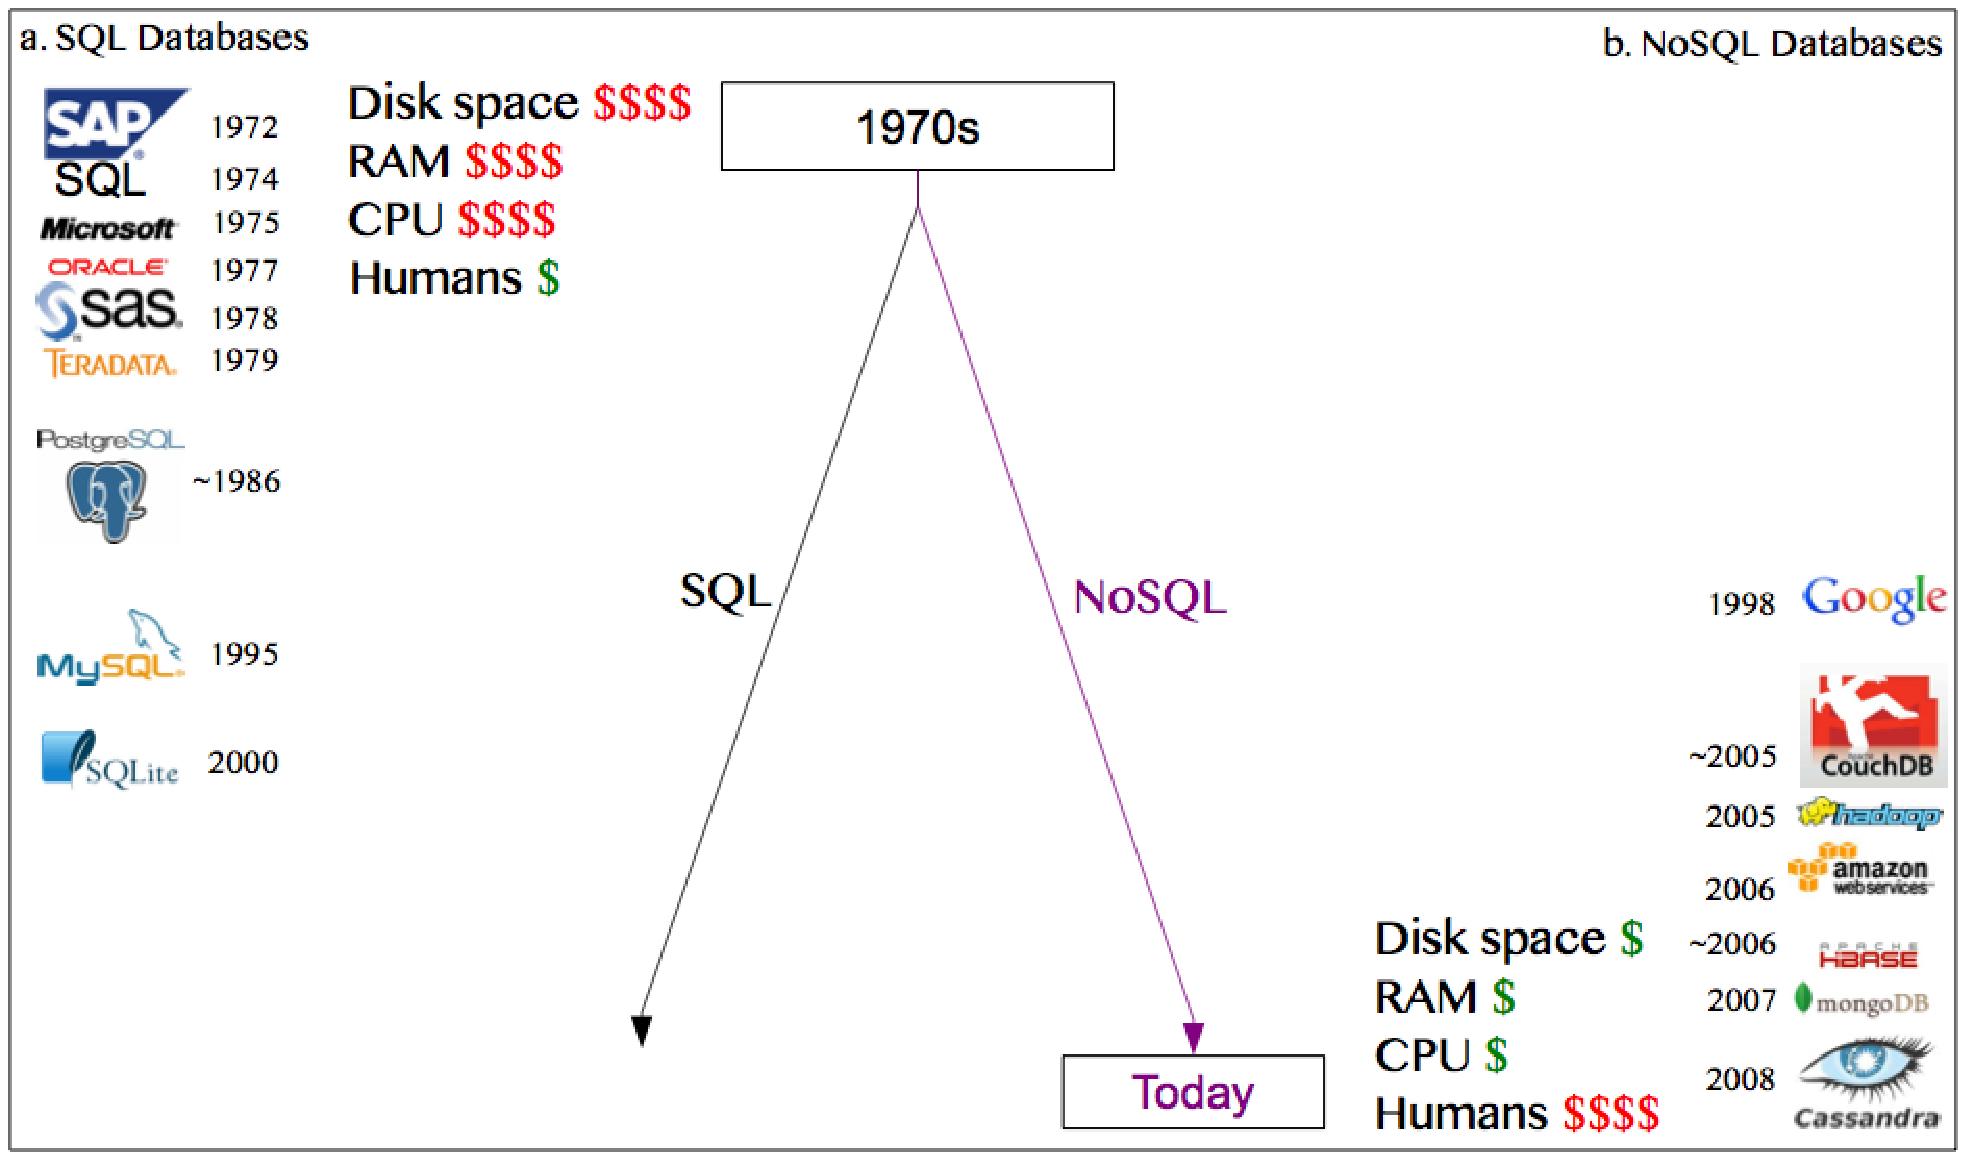
\includegraphics[width=0.8\textwidth]{databasetrends}

\label{ex:databasetrends}
\end{exe}


In June 2012, only one month before we launched the project at CAML, it became possible to build a web app which also worked offline. 
%\footnote{To develop LingSync we had been using a developer edition of Chrome which was two months before normal Chrome.}
 In April 2013 CouchDB added CORS (Cross-Origin Resource Sharing) support,  permitting what are called `mashups' essentially the ability for one to build  independent apps which interfaces with LingSync data securely in realtime, with no additional infrastructure. 

Prior to 2011 there is one other aspect of LingSync which was not possible: only one programming language is used throughout LingSync. The web services are written in JavaScript, the user interface is written in JavaScript, and even the database queries are written in JavaScript. JavaScript has a very simple yet consistent syntax, and only a handful of data types, meaning that research assistants can learn to script in less than one week, and even design and complete their own components in one semester. JavaScript has only recently become a popular programming language, and as such there are a wealth of beginner friendly video screencasts and tutorials which are targeted at non-programmers. Prior to 2011 research assistants frequently learned Python, Bash, and Unix utilities to help clean and transform data,  in addition of course to \LaTeX  and/or Praat. Unlike professional field work, research is unknown, no software can plan everything a research team might wish to do with their data.  As most research budgets are dedicated to funding students, and a growing number of linguistics students come to a department with a basic knowledge of web programming, a viable solution is ask research assistants to manipulate data in batches via scripts. Without a bit of scripting, research assistance are relegated to tasks of monotonous repetition which must be performed in a consistent manner. Training research assistants to script data manipulation not only saves time, but also permits labs to pass on technical knowledge to future lab members, rather than outsourcing  data management to external consultants or computer science students who have largely been trained on SQL best practices which contradict the best practices  needed for smooth data management of the NoSQL data inherent in field work. \cite{Thieberger:2012} also advocates in-house learning, ``there is a need for data management skills to be developed among linguistic scholars so that our relatively small collections can be maintained.''% \citep[p.133]{}   

%It is also worth noting the ability of primary video and audio data to reside in the same system as text data has matured and is as of 2012 is mature enough on all laptops in the form of HTML5 audio and video. \citep{Pfeiffer:2010}.
 
\section{LingSync's Data Model}
\label{appendix:datumjson}

\begin{verbatim}
{
   "_id": "89bc4d7dcc2b1fc9a7bb0f4f474a7fb4",
   "_rev": "7-0d53714bc3b67681892fa0791cbebac3",
   "audioVideo": [],
   "comments": [
       {
           "text": "Hi\nJust a quick note to say that I automatically cleaned this datum. \n\nChanges:\n *  quote encoding problems `We feel like yelling at the children.\" -> We feel like yelling at the children.\n\nExplanation: I was asked by lingllama to come by and standardize quotes today. According to his corpus' convention, we don't need quotes in the translation field.",
           "username": "quotecleaningbot",
           "timestamp": 1389642361952,
           "gravatar": "968b8e7fb72b5ffe2915256c28a9414c",
           "timestampModified": 1389642361952
       }
   ],
   "dateEntered": "\"2013-03-17T23:07:42.760Z\"",
   "dateModified": "\"2013-12-02T20:19:17.321Z\"",
   "datumFields": [
       {
           "label": "judgement",
           "value": "*",
           "mask": "*",
           "encrypted": "",
           "shouldBeEncrypted": "",
           "help": "Grammaticality/acceptability judgement (*,#,?, etc). Leaving it blank can mean grammatical/acceptable, or you can choose a new symbol for this meaning.",
           "size": "3",
           "showToUserTypes": "linguist",
           "userchooseable": "disabled"
       },
       {
           "label": "utterance",
           "value": "Erqekunata noqayku qaparinaywanku.",
           "mask": "Erqekunata noqayku qaparinaywanku.",
           "encrypted": "",
           "shouldBeEncrypted": "checked",
           "help": "Unparsed utterance in the language, in orthography or transcription. Line 1 in your LaTeXed examples for handouts. Sample entry: amigas",
           "showToUserTypes": "all",
           "userchooseable": "disabled"
       },
       {
           "label": "morphemes",
           "value": "Erqe-kuna-ta noqa-yku qapari-nay-wanku",
           "mask": "Erqe-kuna-ta noqa-yku qapari-nay-wanku",
           "encrypted": "",
           "shouldBeEncrypted": "checked",
           "help": "Morpheme-segmented utterance in the language. Used by the system to help generate glosses (below). Can optionally appear below (or instead of) the first line in your LaTeXed examples. Sample entry: amig-a-s",
           "showToUserTypes": "linguist",
           "userchooseable": "disabled",
           "alternates": [
               "Erqekuna-ta noqayku qapari-nay-wanku.",
               "Erqe-kuna-ta noqayku qapari-nay-wanku.",
               "Erqekunata noqayku qaparinaywanku."
           ]
       },
       {
           "label": "gloss",
           "value": "child-PL-ACC 1PL.ex yell-DES-3PL.1PLexOM",
           "mask": "child-PL-ACC 1PL.ex yell-DES-3PL.1PLexOM",
           "encrypted": "",
           "shouldBeEncrypted": "checked",
           "help": "Metalanguage glosses of each individual morpheme (above). Used by the system to help gloss, in combination with morphemes (above). It is Line 2 in your LaTeXed examples. We recommend Leipzig conventions (. for fusional morphemes, - for morpheme boundaries etc)  Sample entry: friend-fem-pl",
           "showToUserTypes": "linguist",
           "userchooseable": "disabled",
           "alternates": [
               "?-ACC ? yell-DES-?",
               "child-PL-ACC ? yell-DES-?",
               "Erqe-kuna-ta noqayku qapari-nay-wanku.",
               "Erqekuna-ta noqayku qapari-nay-wanku."
           ]
       },
       {
           "label": "syntacticCategory",
           "value": "",
           "mask": "",
           "encrypted": "",
           "shouldBeEncrypted": "checked",
           "help": "This optional field is used by the machine to help with search and data cleaning, in combination with morphemes and gloss (above). If you want to use it, you can choose to use any sort of syntactic category tagging you wish. It could be very theoretical like Distributed Morphology (Sample entry: ?-GEN-NUM), or very a-theroretical like the Penn Tree Bank Tag Set. (Sample entry: NNS) http://www.ims.uni-stuttgart.de/projekte/CorpusWorkbench/CQP-HTMLDemo/PennTreebankTS.html",
           "showToUserTypes": "machine",
           "userchooseable": "disabled"
       },
       {
           "label": "translation",
           "value": "We feel like yelling at the children.",
           "mask": "We feel like yelling at the children.",
           "encrypted": "",
           "shouldBeEncrypted": "checked",
           "help": "Free translation into whichever language your team is comfortable with (e.g. English, Spanish, etc). You can also add additional custom fields for one or more additional translation languages and choose which of those you want to export with the data each time. Line 3 in your LaTeXed examples. Sample entry: (female) friends",
           "showToUserTypes": "all",
           "userchooseable": "disabled"
       },
       {
           "label": "tags",
           "value": "Impulsative, Person, Agreement",
           "mask": "Impulsative, Person, Agreement",
           "encrypted": "",
           "shouldBeEncrypted": "",
           "help": "Tags for constructions or other info that you might want to use to categorize your data.",
           "showToUserTypes": "all",
           "userchooseable": "disabled"
       },
       {
           "label": "validationStatus",
           "value": "CheckedWithSeberina",
           "mask": "CheckedWithSeberina",
           "encrypted": "",
           "shouldBeEncrypted": "",
           "help": "For example: To be checked with a language consultant, Checked with Sebrina, Deleted etc...",
           "showToUserTypes": "all",
           "userchooseable": "disabled"
       },
       {
           "label": "dateElicited",
           "value": "5/7/2010",
           "mask": "5/7/2010",
           "encrypted": "",
           "shouldBeEncrypted": "checked",
           "help": "This field came from file import ",
           "userchooseable": ""
       },
       {
           "label": "notesFromOldDB",
           "value": "backwards agreement",
           "mask": "backwards agreement",
           "encrypted": "",
           "shouldBeEncrypted": "checked",
           "help": "This field came from file import ",
           "userchooseable": ""
       },
       {
           "label": "dialect",
           "value": "Cusco Quechua",
           "mask": "Cusco Quechua",
           "encrypted": "",
           "shouldBeEncrypted": "checked",
           "help": "This field came from file import ",
           "userchooseable": ""
       },
       {
           "label": "syntacticTreeLatex",
           "value": "",
           "mask": "",
           "encrypted": "",
           "shouldBeEncrypted": "",
           "help": "This optional field is used by the machine to make LaTeX trees and help with search and data cleaning, in combination with morphemes and gloss (above). If you want to use it, you can choose to use any sort of LaTeX Tree package (we use QTree by default) Sample entry: Tree [.S NP VP ]",
           "showToUserTypes": "machine",
           "userchooseable": "disabled"
       },
       {
           "label": "enteredByUser",
           "value": "",
           "mask": "",
           "encrypted": "",
           "shouldBeEncrypted": "",
           "help": "The user who originally entered the datum",
           "showToUserTypes": "all",
           "readonly": true,
           "userchooseable": "disabled"
       },
       {
           "label": "modifiedByUser",
           "value": "public",
           "mask": "public",
           "encrypted": "",
           "shouldBeEncrypted": "",
           "help": "An array of users who modified the datum",
           "showToUserTypes": "all",
           "readonly": true,
           "users": [
               {
                   "username": "public",
                   "gravatar": "968b8e7fb72b5ffe2915256c28a9414c",
                   "firstname": "",
                   "lastname": ""
               }
           ],
           "userchooseable": "disabled"
       }
   ],
   "pouchname": "lingllama-communitycorpus",
   "session": {
       "sessionFields": [
           {
               "label": "goal",
               "value": "This data was collected by ME Cathcart for her dissertation \"Impulsatives: The syntax and semantics of involuntary desire\" for more of her data: https://github.com/mecathcart/Impulsatives",
               "mask": "This data was collected by ME Cathcart for her dissertation \"Impulsatives: The syntax and semantics of involuntary desire\" for more of her data: https://github.com/mecathcart/Impulsatives",
               "encrypted": "",
               "shouldBeEncrypted": "",
               "help": "This describes the goals of the session.",
               "userchooseable": "disabled"
           },
           {
               "label": "consultants",
               "value": "Lucia, Ricardo, Seberina",
               "mask": "Lucia, Ricardo, Seberina",
               "encrypted": "",
               "shouldBeEncrypted": "",
               "help": "Example from DataOne: Format conventions: use uppercase ,Codes for missing values: unknown",
               "userchooseable": "disabled"
           },
           {
               "label": "dialect",
               "value": "",
               "mask": "",
               "encrypted": "",
               "shouldBeEncrypted": "",
               "help": "You can use this field to be as precise as you would like about the dialect of this session.",
               "userchooseable": "disabled"
           },
           {
               "label": "language",
               "value": "",
               "mask": "",
               "encrypted": "",
               "shouldBeEncrypted": "",
               "help": "This is the langauge (or language family) if you would like to use it.",
               "userchooseable": "disabled"
           },
           {
               "label": "dateElicited",
               "value": "Summer 2010",
               "mask": "Summer 2010",
               "encrypted": "",
               "shouldBeEncrypted": "",
               "help": "This is the date in which the session took place.",
               "userchooseable": "disabled"
           },
           {
               "label": "user",
               "value": "",
               "mask": "",
               "encrypted": "",
               "shouldBeEncrypted": "",
               "help": "Example from DataOne: Format conventions: use uppercase ,Codes for missing values: unknown",
               "userchooseable": "disabled"
           },
           {
               "label": "dateSEntered",
               "value": "",
               "mask": "",
               "encrypted": "",
               "shouldBeEncrypted": "",
               "help": "This is the date in which the session was entered.",
               "userchooseable": "disabled"
           }
       ],
       "pouchname": "lingllama-communitycorpus",
       "comments": [
       ],
       "dateCreated": "\"2013-03-17T23:07:34.194Z\"",
       "dateModified": "\"2013-03-17T23:07:34.194Z\"",
       "timestamp": 1363561654194,
       "_id": "89bc4d7dcc2b1fc9a7bb0f4f474415e4",
       "_rev": "1-701f44686ae45a27d4e5a08ed6c26dc8"
   },
   "timestamp": 1386015557322,
   "jsonType": "Datum",
   "collection": "datums"
}
\end{verbatim}






% The cutting room floor

% was built using tools and practices used for flexible data management which have come out of recent (2005) publications of how to scale flexible and incomplete data from disparate sources. 
%We believe LingSync's position in providing an easy to use tool which produces highly structured data makes it help advance current efforts to assist field work teams to preserve their data.



%linguists are now also much more aware of the need to create records that can be reused by the people we record and that will still be available for their descendants.  \citep[p.129]{Thieberger:2012}
%importance of designing documentary projects in ways that allow speaker communities to benefit from the work of an outside researcher. \citep{Good:2012, }



%The existing linguistic database programs,
% although useful,
% have various shortfalls that would hinder collection and integration of data.
% Some of them are constrained by the internet accessibility or by the computer platform types.
% Some others demand extra human work in order to integrate data.
% Data entry can require hours of a researcherÕs time.


%add discussion of Audiamus by Thieberger?




%The application will be available for any device that has an HTML5 compatible browser, making collaborative work easier among users with different device preferences. 

%As a tool for research, a software should ideally require no time for researchers to learn its functionality.  Various functions in LingSync are organized into widgets (e.g. data entry widget, search widget), and the user interface of each widget transparently reflects its function in order to minimize the time spent on figuring out the behaviour of the application. 
%The database software underlying LingSync (CouchDB) allows data schema to change, which enables researchers to customize and modify data entry fields at any point during the course of research. In addition to the default data fields (utterance, morpheme, gloss, translation) researchers can add `phonetic transcription' or `context of utterance' as data fields, for example. 
%CouchDB has the ability to deal with and record data modifications that happen concurrently by multiple users. LingSync's activity feed widget reports each modification to users who share the same database, making it easy for a team of researchers to keep track of their data and to work on the same database without concern of compromising or losing data. 
%Import and export functions in LingSync allows researchers to gather and organize data that created in different formats, and put them back into a desired format. 
 

%Although it is designed primarily for linguists, the application will equally be useful for researchers documenting endangered languages and/or creating dictionaries/grammar books for minority languages, as well as language teachers creating educational materials.  


%\item {\bf EMELD.} The application will allow researchers to share their data with anyone interested in their work. The application will be able to import data from ELAN XML, CSV and text file formats, and to export to XML, Latex and WIki formats. These import/export functions will make it easier to exchange data with those who are not using the same application.  The system will have users and teams, and permissions for corpora. Permissions will ensure that data can be safely shared and edited by multiple users. Moreover, the corpus will be versioned so that users can track changes and revert mistakes.
%
%
%\item {\bf  Leipzig.} The application will be designed for search as this is one of the most fundamental tasks a language researcher must be able to do. The search will go far beyond traditional string matches and database indexes. The application will guess what users do most often, and automate the process for them. Most importantly, the system will have semi-automated  glossing based on morpheme segmentation.
%
%
%\item {\bf XML/JSON.} Data will be stored on a CouchDB server, and will be accessible and sharable by multiple users.  The installable Chrome extension version of the application allows individual researchers to store a portion of a corpus, or an entire corpus, on their own devices, enabling offline work and quick search. 
%

% The Annotations include three types, free text, enumerated grammatical tags, and enumerated datum validation status (checked with a consultant, to be checked, elicitation error, deleted etc). 



%\begin{verbatim}
% {
%    "_id": "38b751d2a58a13f04a201ac9f95ad5bf",
%    "_rev": "6-e32a664c637415978185bcf2fbb3add9",
%    "audioVideo": {
%        "URL": "",
%        "type": "audio"
%    },
%    "comments": [{
%        "text": "Transliterated from: gen:23:11 ???? ???...?????.? to: gen:23:11 ?aakka an...jiat tavvani iluviliruk.?",
%        "username": "inuktituttransliterationbot",
%        "timestamp": 1377913504452,
%        "gravatar": "968b8e7fb72b5ffe2915256c28a9414c",
%        "timestampModified": 1377913504452
%    }],
%    "dateEntered": "\"2013-06-14T23:10:35.237Z\"",
%    "dateModified": "\"2013-09-25T15:31:53.782Z\"",
%    "datumFields": [
%    ...
%     {
%        "label": "utterance",
%        "value": "?aakka angaju...ni iluviliruk.?",
%        "encrypted": "",
%        "help": "This field is the common writing system for most Inuktitut speakers and may contain transliteration errors, see orthography for the original orthography of the data source.",
%        "userchooseable": "disabled"
%    }, {
%        "label": "gloss",
%        "value": "?-? ? ...?-t ?-? ?-? death-?-t ?-? ?",
%        "encrypted": "",
%        "shouldBeEncrypted": "checked",
%        "help": "This line appears in the gloss line of your LaTeXed examples, we reccomend Leipzig conventions (. for fusional morphemes, - for morpheme boundaries etc) The system uses this line to partially help you in glossing. ",
%        "userchooseable": "disabled",
%        "alternates": [
%            "?-? ? ? ? ? ...?-t ?-?-t ?-? ?-? death-?-t ?-? ?",
%            "?-aakka angajuqkaak, na...-jia-t tavva-ni iluviliruk.-?",
%            "?-aakka angajuqkaak, naa.-jia-t tavva-ni iluviliruk.\""
%        ]
%    }, {
%        "label": "orthography",
%        "value": "???? ??????, ????....??.?",
%        "encrypted": "",
%        "shouldBeEncrypted": "checked",
%        "help": "This field was from the original data source, it was transliterated using a script to create the utterance line.",
%        "userchooseable": "enabled"
%    }
%    ...
%    ],
%    "timestamp": 1380123113782,
%    "jsonType": "Datum",
%    "collection": "datums"
%}
%
%\end{verbatim}


%The system is designed not only for data entry, but also for data retrieval. 
%Furthermore, data stored in the application, if the field tagged as public by the researcher, is indexable by search engines and open to public view in principle. However, authorized researchers (authors of data) have control over who can see, edit and/or export their data.  
% Confidential data are stored encrypted in the database. 
%The application allows two sorts of export. Export of encrypted output maintains encryption on confidential data, allowing researchers to make their public data public, without concern that confidential data or consultant information will become public. Export of decrypted output keeps the data non-proprietary and viewable outside of the app and must be protected as any other confidential data. 


%As endangered language data may often have a condition of being kept private until its parties have passed away, should the administration member of the corpus die, a policy of obeying his/her heir's decisions with regard to the data shall be put in place and discussed in the terms and conditions. 





%\subsubsection{DataONE Primer on Data Management} 
%
%DataONE provides guidelines for data management according to 8 stages of data life cycle. Although the guidelines are primarily directed to researches in natural sciences, they are also relevant for linguistic research and language documentation.  
%
%\begin{description}
%
%%\item { \bf OpenSource}. Being OpenSource allows departments to install and customize the database application to tailor their specific needs without worry that the company behind the software will disappear or stop maintaining the software. In addition, OpenSourcing the software on GitHub will allow linguists with scripting or programming experience to contribute back to the software to make it more customized to their needs, language typologies, or linguistics research areas. It allows the software to continue to grow and improve without any company which seeks to profit from the software.
% 
%
%%\item {\bf OpenAccess}. Corpora often contain sensitive information, consultant stories and other information which must be kept confidential. Having confidential data in plain text in a corpus forces the entire corpus to be kept confidential. Instead, the system will encrypt confidential data and store the data in the corpus encrypted. To access the plain text the user will have to log in and use a password to decrypt the data. This design has important ramifications for exporting data, and for editing the data outside the application. The system will allow the user to export data encrypted or decrypted. If the corpus contains sensitive confidential information the system will warn the users if they choose to export the information in a decrypted fashion.
%
%
%
%%\subsubsection{Standards-compliant (Unicode, EMELD, Leipzig, XML)}
%
%% Audio files will be stored elsewhere (not on a CouchDB server), most likely on researcher's own server, to keep the storage space small in order to provide . The database will contain the information of the location path of the audio files, and when users want to access audio files, they will be redirected to their location. We'll use Iris CouchDB which provides free service if the usage (storage and transaction) is less than 5$/month (http://www.iriscouch.com/service). If we host only text data, it is possible to keep the service free. 
%
%
%
%\item {\bf Plan}: Plan for data management prior to data collection and revise it as necessary during the project. 
%
%
%%LingSync can be used to plan and manage data collection process. Users can begin by adding a description to their corpus, as well as adding language consultants and collaborators. When they begin collecting data they are first prompted to enter a Session and encouraged to write the session goals. Users are even able to prepare hypotheses in the form of Data lists containing Datum "To be Checked" to prepare for their data elicitation session with their language consultant. In this way LingSync helps a researcher in their collection rationale, collection and analysis methods. When the users add fields to datum they can enter a help text which will pop-up over the datum field as users are entering if they need to know what are the conventions for that field, e.g. IPA transcription could be either phonological or phonetic, the corpus administrator can indicate the conventions using the help text. 
%
%LingSync is designed in consideration of concerns users would encounter when planning to create language databases. 
%
%
%\begin{itemize} 
%
%\item{\sc Repository}: Data can be stored on cloud servers or on department or institution's own servers. Users can also store their databases on their own devices. Depending on the cyberinfrastructure available to users, LingSync allows flexible repository choices. 
%
%\item{\sc Data organization}: Data is stored in a versioned document-centered storage solution referred to as "NoSQL." Data is stored in JSON format (exportable to .csv, .xml, .txt, .tex). Unlike SQL databases, NoSQL databases are designed to expand limitlessly, to allow data schema to change and to provide powerful search of data in context.
%
%\item{\sc Data management}: LingSync allows number of permissions for data access and management. All data are versioned and data history is easily trackable, which enables users to recover and resolve mistakes or inconsistent annotation. Comment feeds on datums encourage users to discuss issues they discover on their data.   
%
%\item{\sc Data description}: A datum is produced according to Leipzig conventions, and LingSync provides four data fields (utterance, morphemes, gloss, translation) as default. Additional metadata description are configured on a corpus basis by the corpus administrator. (See also Collect below.)
%%LingSync offers a list of commonly used annotation fields to researchers which is generated by the popularity of fields among app users. 
%
%\item {\sc Data sharing}: Data may be shared with members of a research team through access permissions. Data may also be converted to commonly used formats (.csv, .xml, .txt, .tex) to be given directly to members who are not using LingSync. Users can also embed live widgets to share portions of data on project's webpages, or WordPress blogs. Users can schedule "Bots" to automatically release/publish their data to external web services or language archives.
%
%\item{\sc Data preservation}: As mentioned in {\sc Repository} above, data can be stored on a central server of user's choosing or on users' own devices. In addition "Bots" have been included as a feature so that users can automatically archive their data in existing, reputable language data archives. (See \S \ref{sec:documentation} Preservation) Multiple storage locations means less risk of losing data.
%
%
%\item{\sc Budget}: LingSync is free and OpenSouce. The application can be installed for free on department servers or institutional data centres, which may require hiring professionals to maintain the database and ensure that the data is properly backed up. LingSync can also run on the cloud and departments can choose to host their data on a cloud hosting provider. The costs usually range between \$1 and \$10 per month for 1-100 gigabytes of data/data transfer.
%
%\end{itemize} 
%
%LingSync can also be used to plan and manage data collection process. Users can begin by adding a description to their corpus, as well as adding language consultants and collaborators. When they begin collecting data they are first prompted to enter a Session and encouraged to write the session goals. Users are even able to prepare hypotheses in the form of Data lists containing Datum "To be Checked" to prepare for their data elicitation session with their language consultant. In this way LingSync helps a researcher in their collection rationale, collection and analysis methods. When the users add fields to datum they can enter a help text which will pop-up over the datum field as users are entering if they need to know what are the conventions for that field, e.g. IPA transcription could be either phonological or phonetic, the corpus administrator can indicate the conventions using the help text. 
%
%
%\item {\bf Collect}: Data is collected in such a way to ensure future usability.\footnote{DataOne recommends plain text ascii characters for variable names, file names, and data. As ascii is inappropriate for linguistic data, we follow E-MELD's recommendation to ensure that orthography, IPA, diacritics, semantic calculations and other are maintained in our users data.}
%
%
%The application provides a template for data entry which is flexible and customizable. The four core data fields (utterance, morphemes, gloss, translation) are usually required for language data and are set as defaults on the template. Researchers can add extra fields (e.g. IPA transcription, context of utterance) relevant to their research. Each data field has an optional Help Text where users can add detailed description of the data content. Contents of data fields (default and additional) are object of Search function so that users can organize data using the information contained in the fields. Search results can be made into and stored as independent data lists. 
%
%The application is non-proprietary and data collected are exportable in various formats (.csv, .xml, .txt, and .tex) to ensure that data is sharable and usable outside the application. 
%When the user exports their corpus a readme.txt is generated which describes the datum annotation fields (using the conventions help text which the users can customize). In this way, when they share their data they can attach the readme.txt to allow others to know what their conventions were when building their corpus. 
%
%
%
%\item{\bf Assure}: The quality of data is assured through checks and inspections. 
%
%Datum's validation status (Checked, To be checked, Elicitation Error) and datum comment feeds enable users to check, discuss and inspect the data quality.  
%%Each datum is associated with session information such as researcher's name, consultant's code and date of elicitation. 
%Each datum is also time stamped when entered and modified so that the data history is trackable. Users may also create "Bots" which crawl their data and ensure that it is consistent.
%
%% Each modification is recorded (I think) but the app would only show last modified ? 
% 
%\item{\bf Describe}: Data is accurately and thoroughly described using the appropriate metadata standard.  
%
%Data will be described at three levels in the application: 
%
%\begin{itemize} 
%\item Corpus: A corpus is a dataset created for a single language/dialect and for a particular purpose. A corpus has a title and a description that will include general information about the corpus such as what the dataset is about, who contributes to the corpus and the purpose of creating the corpus.  
%\item Session: Each datum in a corpus is tied to a Session which includes metadata such as language, dialect, researcher's name, consultant's code and the goal of the session (e.g. eliciting scope ambiguity).  
%\item Datum: Data fields and data tags serve for parameters/categories to describe data. The application is not restricted to a particular theoretical construct so that researchers can choose categories appropriate to their research, and describe the categories using Help Text. (See also Collect above)
%% describe categories -- I meant the hint pop-up box for extra datum field where users can give hints what should be in the field. 
%\end{itemize} 
%
%
%
%\item{\bf Preserve}: Data is submitted to an appropriate long-term archive.  
%
%Data and associated metadata are stored in a host server for long-term archival purposes. Confidential data and information are stored encrypted using the US Federal approved AES encryption standard to ensure that confidential data cannot be leaked if a corpus is shared or leaked, without the consent of the corpus' author. (See also \S \ref{sec:documentation} Citation, Preservation \& Rights)
%
%
%\item{\bf Discover}: Data is located and obtained. 
%
%The data in LingSync, if tagged for public view, are in principle searchable via standard search engines. Data permitted for export will be exportable to CSV, XML, text or LaTex formats. (See also \S \ref{sec:documentation} Discovery, Access \& Citation)
%
%\item{\bf Integrate}: Data from disparate sources are combined into one consistent data set. 
%
%LingSync can be used to integrate and organize data created in different applications. Import/Export functions enable to combine data created in different file formats (e.g. .csv from FileMaker Pro and .xml from ELAN) into .json files and export them back to the original formats. While on LingSync, data can be made consistent by the creation of "Bots" who crawl the corpus and automate changes.
%
%\item{\bf Analyze}: Data is analyzed. 
%
%The four core data fields include morpheme-segmentation and glossing lines, hence the data will contain primary linguistic analysis at the time of the entry to the database. 
%Customizable data entry fields and data tags, as well as the data list  functionality allows researchers to organize data ready for further analysis.   
%
%\end{description} 


%
%
%
%
%
%
%
%
%
%The usefulness and effectiveness of the iFiled App will be evaluated against the following criteria, taken and modified from E-MELD Best Practices in Digital Language Documentation (http://emeld.org/school/what.html) and DataONE Primer on Data Management (http://www.dataone.org/sites/all/documents/DataONE\_BP\_Primer\_020212.pdf). 
%
%\begin{enumerate} 
%
%\item Collection: Data are collected and organized with ease. 
%
%Self-explanatory UI as well as online and offline functionality will make data collection easier.   This is a fundamental difference between LingSync, designed by field linguists with software engineering experience, and existing databases which were designed by computer science students, or programmers with no fieldwork experience.
%
%\item Quality: The quality of data is assured. 
%
%Datum state (Checked, to be checked, Elicitation Error) and datum comment feeds enables researchers to check and inspect the data quality.  
%
%\item Description: Data are annotated and categorized according to various terminological conventions.  \\ Data fields and tags accommodate metadata categories and  are customizable by corpus teams, for their team's corpora. The application thus allows data to be annotated and categorized, without unneccessarily  reducing the ease of data entry. 
%
%\item Integration: Data from disparate sources are combined into one consistent data set. \\ Sync function helps integrate data taken by multiple researchers into one corpus. Import/export functions enables integration of data from Filemaker Pro (.csv) and ELAN (xml), making data integrated with programs researchers commonly use/have used to store their data.
%
%\item Analysis: The application organizes data in ways to help data analysis. \\  Customizable data entry fields and data tags, as well as the data list  functionality allows researchers to organize data ready for analysis.  
%
%\item Format: Data are intelligible regardless of the types of operating system. (E-MELD Summary of Best Practices 2)
%
%The application runs on PC, Linux and Mac OS, as well as on newer platforms such as Android and ChromeBook. The application supports Unicode and exportable to .json, .tex, .txt, .csv, and .xml files. The application allows export of encrypted  output, allowing researchers to make their public data public, without concern that confidential data or consultant information will become public, or export of decrypted output which keeps the data non-proprietary and viewable outside of the app.
%
%\item Discovery: Data are searchable and discoverable. \\ The application is accessible through general internet search. Within the application, data are discoverable via keyword search. The two-step data discovery process will minimize irrelevant search results.   
%
%\item Access: Data are accessible. \\ Data stored in the application, if tagged as public by the researcher, is indexable by search engines and open to public view in principle, however authorized researchers (authors of data) have control over who can see and/or edit their data. 
%
%\item Citation: Data provide citation information. \\ All data points are tied to a Session which contains details of data source such as consultant, publication, web page in addition to the time the data was entered and other metadata controlled by the researcher to ensure that data quality can be traced to its source.
% 
%\item Preservation: Data are archived in a way that withstands long-term preservation. \\ Data are stored in a host server as JSON files. JSON files are human-readable text files, therefore the information content would not be lost even if the data format becomes obsolete. 
%
%\item Security: Confidential information must be kept from public access. \\ Data tagged as confidential, as well as consultant information which is confidential are encrypted in the database using the US Federal approved AES encryption standard. This ensures that confidential data cannot be leaked if a corpus is shared or leaked, without the consent of the corpus' author. 
%
%\end{enumerate} 


%
%Provide information on the metrics that will be used to determine the effectiveness of the project. It has to meet certain data management criteria -- any scientist can discover and use the data over time; it will benefit the scientific community. We are abiding by the best practice standards set by DataOne.   
%
%Example format: 
%
%\exg. n-tuop'ti-m\\
%1-window-POSS.SG\\
%`My window'
%
%


%\subsubsection{User-friendly}


%\begin{description}
%\item { \bf Simple.} The system will be designed to replace Word Documents or LaTeX documents which is a very common way field linguists store data because it requires no training, doesn't require a complicated set-up for data categories, and takes no time to add new categories.  The application will not include categories or linguistic frameworks or theoretical constructs that must be tied to the data.  The application will allow data fields and categories to develop organically as data collection proceeds, as opposed to imposing a particular construct upon entry.  Researchers will be able to add and change their fields and categories for the data at any point.

%\item {\bf Attractive.} The system will have a modern design like many of the popular websites such as Google and Twitter. It's layout and background image will be customizable so that the user can change the look and feel of the application to make their eyes comfortable  in bright/dark light, or adapt the layout of the widgets to their style of data entry.

%\item { \bf Cross-Platform.} The application will be available for any device that has an HTML5 compatible browser. Specifically, the application will run \emph{offline/online} in Chrome  on Mac, Linux, and Windows computers,\footnote{The app will also run on ChromeBooks. ChromeBooks are affordable laptops (\$299) which use the Chrome operating system created by Google. ChromeBooks are currently available in the UK and online at www.google.com/chromebook/. ChromeBooks have very long battery life and automatically backup data, which makes them good laptops for fieldwork.} as well as \emph{online/online} on Android tablets and phones. The application will run \emph{online only} in Safari and Firefox, and \emph{online only }on iPads and iPhones. 
% As of June 28 2012, Chrome runs on iPads and iPhones. Accordingly the application will run both online and offline on iPads and iPhones.  

%Touch tablets are one of the easiest tools to carry and use in the field; they have a long battery life; they can play videos or show images for the consultant to elicit complicated contexts; and they permit recording audio and video without  microphones or cameras which distract consultants. Mobile devices also have apps for push button  publishing to YouTube or other audio/video hosting solutions  which  allow for private data like Google Plus. Furthermore, Android tablets are particularly easy to program and integrate the microphone/camera directly into the database (Cook, Marquis and Achim 2011).
%


%\item {\bf Work offline.} Running a webapp offline will have considerable consequences for how data is stored, how data is retrieved, and how much data can be used while offline. Most browsers have limits on the amount of data a webapp can store offline. By delivering a version of the application in a Chrome extension, which has permission to have unlimited storage, researchers will be able to have a significant portion of their data at their fingertips, regardless of the location. 

%\end{description}



% The dashboard usually composed of several widgets.
%%true for the prototype but do we want to talk about that or about the spreadsheet one? 
% The Data Entry widget is the primary focus,
%containing four core fields customary for a gloss format (utterance,
%morpheme-segmentation,
%gloss,
%translation).
%In addition to these fields,
%researchers can add custom fields,
%such as phonetic transcription or context for an utterance.
% Researchers can even record or upload audio files directly into the appropriate data record.
%Each data entry is  tagged with session info such as the who entered the data,
%who participated in the data collection,
%the date of elicitation,
%the language,
%dialect and consultant's code.


% with an unexpected number of users, to date (January 2014) LingSync now has over 300 users who have created over 1000 databases.


% The core features are summarized in the following subsections.
 


% ``structure proposed does not appear at the surface to permit the fluidity needed in changing categories and labels as an analysis changes.'' \citep[p.11]{Cihlar:2008}. 
%

%In our experience as field work research assistants we estimate that well over 50\% of research time is spent cleaning and curating data,
%often to revise old data to update it to the team's evolving analysis.




%TODO discuss elan import...
%see \cite{Schroeter:2006}p105 



%Currently,
%there is no user interface to view/edit a corpus' lexicon but if there is enough demand it will prioritized.





%\begin{exe}
%	\ex Search for  `nay[tk]' in the morphemes line to find context of allomorphy
%\end{exe}



%\begin{exe}
%	\ex Search for  `nay-voice' in the morphemes line to find context of surface vowels
%\end{exe}

%Search has a 
%The phonological search module shown in Table~\ref{tab:phono} is used to search for phonological features in context.


%Sample licences which projects can use:
%
%``Photographs, recordings, texts, and work posted here may be used by the Yurok Tribe and other Yurok tribal groups, and may be used by individuals for personal, educational, and scholarly purposes only. No material posted here may be used for any commercial purpose or reproduced without the permission of its author.'' \citep{Yurok:2001:Online}



%discuss Existing data management systems \cite{Schroeter:2006} LACITO and EthnoER as well as the LDC and OLAC...
%and maybe how LingSync data can be imported by them?


% Human factors and Human Computer Interaction and click intensive user interfaces can can often play a larger role in over all time it takes to complete of data entry,
% greatly reducing the positive effects of any tools we can provide to make semi automatically annotate data.
% \citep{Palmer:2010} \citep{Palmer:2009}.

%We have added many other options to corpora which conform to EMELD recommendations discussed in \S\ref{sec:design}.


%and if the software provides a javascript or HTML5 library or widget,




%\subsubsection{Wiki-dictionary format export}

%It is possible to download the entire Wiktionary for a language and import or export it using LingSync  The dictionary module shown in Table~\ref{tab:dictionary} is used to crawl the corpus to gather citations and examples to build a Wiktionary dictionary for the corpus' language,
% as required by some grants which focus on endangered/minority languages.
% The dictionary module is quite complex and the central component of many online fieldlinguistics databases.
	

%\subsubsection{Using LingSync to power online language documentation sites/mobile apps}
%
%\cite{Good:2012}

%\subsubsection{Other}

%\subsection{Collaborators } 
%
%LingSync is a product of collaboration between field linguists,
%programmer linguists,
%and programming field linguists,
%as well as linguistics students who have been trained to code and subsequently contributed to the app.
%
%
%--> perhaps Gina you could talk more about this? Maybe move to the next section with other types of people? 


%(Server logs show the developers logging in and saving activity but not the content of the data.) 



%While more field database tools may surface in the coming years, we believe LingSync to be the only language documentation tool to take advantage of an established scalable NoSQL database solution, rather than reinventing a custom XML data store or relational database schema. 
